% !TeX root = ../main.tex
% Zeile 1 legt fest das immer die main.tex kompiliert wird

%   _________Kapitel 0_________
\chapter{Einleitung}
Diese Arbeit befasst sich mit der Konzeptionierung, Entwicklung und dem Bau einer Wortuhr mit zusätzlichen informativen Funktionen. 
Dabei werden sowohl technische als auch konstruktive und gestalterische Aspekte betrachtet. 

Die Darstellung der Uhrzeit stellt eine grundlegende Funktion technischer Systeme im Alltag dar. 
Neben analogen und digitalen Anzeigen existieren alternative Konzepte der Zeitdarstellung. 
Eine Wortuhr stellt die Uhrzeit in sprachlicher Form dar. 
Dabei werden einzelne Wörter gezielt beleuchtet, sodass eine lesbare Zeitangabe entsteht. 

Im Bereich der Elektrotechnik vereint eine Wortuhr mehrere Fachdisziplinen. 
Hierzu zählen insbesondere Mikrocontrollertechnik, digitale Signalverarbeitung die Integration externer Datenquellen. 
Zusätzlich spielen Aspekte wie Vernetzung, Benutzerinteraktion und Systemintegration eine Rolle. 

Die Entwicklung technischer Systeme erfordert ein strukturiertes Vorgehen. 
Neben der funktionalen Auslegung sind auch Anforderungen an Zuverlässigkeit, Energieeffizienz, Erweiterbarkeit und Gestaltung zu berücksichtigen. 
Eine systematische Konzeption bildet daher die Grundlage für eine zielgerichtete Umsetzung. 
    \input{inhalt/textkapitel/Kapitel 0/010_Motivation und Problemstellung.tex}
    \section{Zielsetzung der Arbeit}
Ziel dieser Arbeit ist, die Konzeptionierung, Entwicklung und den Aufbau einer Wortuhr mit zusätzlichen informativen Funktionen. 

Die Wortuhr soll die Uhrzeit weiterhin in sprachlicher Form darstellen. 
Zusätzlich wird eine sekundengenaue Zeitinformation vorgesehen. 
Darüber hinaus soll das System externe Daten verarbeiten und ausgewählte, informative Zusatzinformationen anzeigen. 

Die Architektur soll so ausgelegt werden, dass eine Einbindung in vernetzte Strukturen möglich ist. 
Ebenso soll eine externe Steuerung und Überwachung über ein mobiles Endgerät realisierbar sein. 

Die Zielsetzung umfasst sowohl die Auslegung der elektronischen Hardware als auch die Entwicklung der notwendigen Software. 
Weiterhin wird die mechanische Konstruktion der Gehäuse- und Trägerelemente berücksichtigt. 
Am Ende der Arbeit steht ein funktionsfähiger Prototyp, dessen Eigenschaften systematisch geprüft und bewertet werden.
    \input{inhalt/textkapitel/Kapitel 0/030_Projektgegenstand und Abgrenzung.tex}

%   _________Kapitel 1_________
\chapter{Marktanalyse und Relevanz des Projekts}

    % \section{Markt- und Wettbewerbsanalyse}
Die Marktanalyse kommerzieller Wortuhren dient der systematischen Untersuchung bestehender Produkte im Hinblick auf technische, funktionale und gestalterische Eigenschaften. 
Ziel ist die Identifikation aktueller Lösungsansätze, technologischer Standards sowie bestehender Einschränkungen. 
Die Analyse bildet eine fundierte Grundlage für die Ableitung eigener Systemanforderungen und unterstützt die Abgrenzung des geplanten Entwicklungsumfangs.

Der Markt für Wortuhren lässt sich grundsätzlich in mehrere Segmente unterteilen, die sich hinsichtlich Designanspruch, Funktionsumfang und Preisniveau unterscheiden. 

Im Premiumsegment dominieren Produkte wie die QLOCKTWO EARTH 45 des Herstellers Biegert\&Funk, die primär als Designobjekte positioniert sind~\cite{qlocktwo_earth45}. 
Diese Uhren bewegen sich typischerweise in einem Preisbereich von etwa 1.500 € bis über 3.000 €, abhängig von Größe und Materialausführung. 
Sie zeichnen sich durch hochwertige Materialien, minimalistische Gestaltung und eine klare Fokussierung auf die wortbasierte Zeitanzeige aus. 
Erweiterte Funktionen wie Wetterinformationen, Sensorintegration oder kontextbasierte Zusatzinformationen sind in diesem Segment kaum vorhanden. 
Trotz des hohen Preisniveaus resultiert daraus ein begrenzter funktionaler Mehrwert.

\begin{figure}[H]
	\centering
	
\includegraphics[width=0.5\linewidth]{inhalt/bilder/QlockTwoDessert.png}
	\caption{}
	\label{fig:qlocktwo_earth45}
\end{figure}

Im mittleren Preissegment finden sich technisch erweiterte Lösungen von Herstellern wie Build-Yours oder kleineren Anbietern im Bereich individualisierbarer LED-Wortuhren. 
Ein Beispiel hierfür ist die Wortuhr Jupiter, die je nach Ausführung in einem Preisbereich von etwa 200 € bis 600 € liegt~\cite{wordclock_jupiter}. 
Diese Systeme erweitern die klassische Wortuhr um grundlegende Funktionen wie WLAN-Anbindung, App-Steuerung oder Farbkonfiguration. 
Dadurch wird insbesondere die Individualisierung der Anzeige verbessert. 
Der Funktionsumfang bleibt jedoch überwiegend auf die Darstellung der Uhrzeit sowie visuelle Anpassungen beschränkt, während eine weitergehende Informationsintegration, beispielsweise durch externe Datenquellen, nur eingeschränkt umgesetzt wird.

\begin{figure}[H]
	\centering
	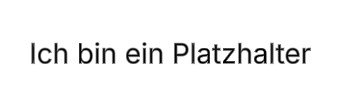
\includegraphics[width=0.5\linewidth]{inhalt/bilder/Platzhalter.jpg}
	\caption{}
	\label{fig:wordclock_jupiter}
\end{figure}

Demgegenüber stehen DIY- und Maker-Lösungen, die auf Mikrocontroller-Plattformen wie dem ESP32 basieren. 
Diese Systeme entstehen häufig in Community-getriebenen Projekten oder individuellen Entwicklungen. 
Die Materialkosten bewegen sich typischerweise im Bereich von etwa 50 € bis 200 €, abhängig von Komponenten wie LED-Matrix, Gehäuse und Sensorik. 
Diese Lösungen ermöglichen eine nahezu beliebige Erweiterung der Funktionalität, etwa durch die Einbindung von Wetterdaten, Temperaturmessung oder weiteren API-basierten Informationen~\cite{esp32_wordclock}. 
Allerdings weisen diese Systeme häufig Defizite hinsichtlich Gehäusedesign, Benutzerfreundlichkeit und Produktreife auf, wodurch sie für eine breitere Zielgruppe nur eingeschränkt geeignet sind.

\begin{figure}[H]
	\centering
	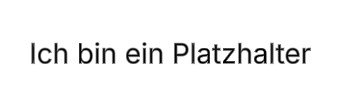
\includegraphics[width=0.5\linewidth]{inhalt/bilder/Platzhalter.jpg}
	\caption{}
	\label{fig:esp32_wordclock}
\end{figure}

Ein weiteres Segment bilden günstige Massenmarktprodukte, die über Onlineplattformen wie Alibaba oder vergleichbare Anbieter vertrieben werden~\cite{alibaba_wordclock}. 
Diese Produkte liegen preislich meist im Bereich von etwa 10 € bis 150 € und zeichnen sich durch eine einfache technische Umsetzung sowie eine stark reduzierte Funktionalität aus. 
Sie sind primär als dekorative Produkte einzuordnen und weisen sowohl in Bezug auf Materialqualität als auch Funktionsumfang deutliche Einschränkungen auf.

\begin{figure}[H]
	\centering
	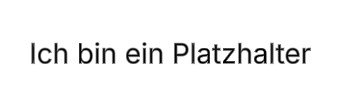
\includegraphics[width=0.5\linewidth]{inhalt/bilder/Platzhalter.jpg}
	\caption{}
	\label{fig:alibaba_wordclock}
\end{figure}

Zur systematischen Bewertung der betrachteten Systeme werden selbst definierte Kriterien verwendet. 
Neben funktionalen Eigenschaften werden der Kaufpreis sowie gestalterische Merkmale analysiert. 
Hierzu zählen insbesondere Materialwahl, Lichtcharakteristik, Formfaktor und Integrationsfähigkeit in Wohnumgebungen. 
Ein weiteres Kriterium stellt die zeitliche Präzision dar. 

Die Gegenüberstellung ermöglicht die Identifikation von Gemeinsamkeiten und Unterschieden zwischen den betrachteten Systemen. 
Auf dieser Grundlage lassen sich funktionale Defizite sowie Potenziale für Erweiterungen ableiten. 
Die gewonnenen Erkenntnisse fließen in die Konzeptionierung der im Rahmen dieser Arbeit entwickelten Wortuhr ein. 
Die Ergebnisse sind tabellarisch in Tabelle~\ref{tab:vergleich_wordclock_ohne_diy} dargestellt.

\begin{table}[h]
\centering
\begin{tabular}{|p{4cm}|p{3.5cm}|p{3.5cm}|p{3.5cm}|}
\hline
\textbf{Kriterium} & \textbf{Premium (z.\,B. QLOCKTWO / Biegert \& Funk)} & \textbf{Mittleres Segment (z.\,B. Build-Yours / Jupiter)} & \textbf{Massenmarkt (z.\,B. Alibaba)} \\
\hline
Preisbereich & ca. 1.500 € – 3.000 € & ca. 200 € – 600 € & ca. 10 € – 150 € \\
\hline
Zielsetzung & Designobjekt / Lifestyle & Kombination aus Technik \& Design & Dekorationsprodukt \\
\hline
Wortbasierte Zeitanzeige & o & o & o \\
\hline
Materialqualität & Sehr hoch (Metall, Holz) & Mittel bis hoch & Niedrig \\
\hline
Designfokus & Sehr hoch & Mittel & Gering \\
\hline
WLAN / Internet & x & o & x \\
\hline
App-Steuerung & x & o & x \\
\hline
Farb- / Anzeigeanpassung & x / sehr begrenzt & o & o (begrenzt) \\
\hline
Sekundenanzeige & o (teilweise) & x & x \\
\hline
Wetterdaten & x & x & x \\
\hline
Temperaturanzeige & x & x & x \\
\hline
Mondzeiten / Zusatzinfos & x & x & x \\
\hline
Erweiterbarkeit (APIs) & x & x & x \\
\hline
Benutzerfreundlichkeit & Sehr hoch & Hoch & Mittel \\
\hline
Produktreife & Sehr hoch & Hoch & Mittel \\
\hline
\end{tabular}
\caption{Vergleich verschiedener Wortuhren in verschiedenen Preissegmenten.}
\label{tab:vergleich_wordclock_ohne_diy}
\end{table}

Aus der Gegenüberstellung ergibt sich eine Diskrepanz zwischen Designqualität und funktionaler Leistungsfähigkeit. 
Im Premiumsegment zeigt sich trotz hoher Preise ein eingeschränkter Funktionsumfang.
Bei der QLOCKTWO CLASSIC ist z.B. eine Sekundenanzeige grundsätzlich möglich, erfordert jedoch dass diese durch drücken eines Knopfes ein- und ausgeschalten wird.
Die Sekundenanzeige erscheint dann als Ziffer durch gezieltes setzen der LEDs auf der Buchstabenmatrix, wodurch die Stundenanzeige unterbrochen ist~\cite{QlockTwoClassicSekundenanzeige}. 
Systeme im mittleren Preissegment bieten erste Ansätze technischer Erweiterungen, erreichen jedoch keine umfassende funktionale Integration moderner Informationssysteme. 
DIY-Systeme weisen eine hohe Funktionalität und Flexibilität bei vergleichsweise geringen Kosten auf, erfüllen jedoch häufig nicht die gestalterischen und konstruktiven Anforderungen eines marktfähigen Produkts.

% %%%%%%%%%%%%Unbearbeitet version, outdated, später löschen sobald neue abgenommen
% \section{Markt- und Wettbewerbsanalyse} \todo{text}
% Die Marktanalyse kommerzieller Wortuhren dient der Untersuchung bestehender Produkte im Hinblick auf technische, funktionale und gestalterische Eigenschaften. 
% Ziel ist die Identifikation aktueller Lösungsansätze, technologischer Standards sowie bestehender Einschränkungen. 
% Die Analyse bildet eine Grundlage für die Ableitung eigener Systemanforderungen und unterstützt die Abgrenzung des geplanten Entwicklungsumfangs.

% Der Markt für Wortuhren lässt sich grundsätzlich in mehrere Segmente unterteilen,die sich vor allem hinsichtlich Designanspruch, Funktionsumfang und Preisniveau unterscheiden. 
% Im Premiumsegment dominieren Produkte wie die QLOCKTWO EARTH 45 des Herstellers Biegert\&Funk, die primär als Designobjekte positioniert sind~\cite{qlocktwo_earth45}.
% Diese Uhren bewegen sich typischerweise in einem Preisbereich von etwa 1.500 € bis über 3.000 €, abhängig von Größe und Materialausführung. 
% Sie zeichnen sich durch hochwertige Materialien, minimalistische Gestaltung und eine klare Fokussierung auf die wortbasierte Zeitanzeige aus. 
% Erweiterte Funktionen wie Wetterinformationen, Sensorintegration oder kontextbasierte Zusatzinformationen sind in diesem Segment kaum vorhanden.
% Trotz des hohen Preisniveaus bieten diese Systeme somit nur einen begrenzten funktionalen Mehrwert.

% \begin{figure}[H]
% 	\centering
% 	
\includegraphics[width=0.5\linewidth]{inhalt/bilder/QlockTwoDessert.png}
% 	\caption{}
% 	\label{fig:qlocktwo_earth45}
% \end{figure}

% Im mittleren Preissegment finden sich zunehmend technisch orientierte Lösungen von Herstellern wie Build-Yours oder kleineren Anbietern im Bereich individualisierbarer LED-Wortuhren. 
% Ein Beispiel hierfür ist die Wortuhr Jupiter, die je nach Ausführung in einem Preisbereich von etwa 200 € bis 600 € liegt~\cite{wordclock_jupiter}. 
% Diese Systeme erweitern die klassische Wortuhr um grundlegende Funktionen wie WLAN-Anbindung, App-Steuerung oder Farbkonfiguration. 
% Dadurch wird insbesondere die Individualisierung der Anzeige verbessert. 
% Dennoch bleibt der Funktionsumfang meist auf die Darstellung der Uhrzeit sowie visuelle Anpassungen beschränkt, während weitergehende Informationsintegration, beispielsweise durch externe Datenquellen, nur eingeschränkt umgesetzt wird.

% \begin{figure}[H]
% 	\centering
% 	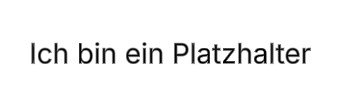
\includegraphics[width=0.5\linewidth]{inhalt/bilder/Platzhalter.jpg}
% 	\caption{}
% 	\label{fig:wordclock_jupiter}
% \end{figure}

% Demgegenüber stehen DIY- und Maker-Lösungen, die auf Mikrocontroller-Plattformen wie dem ESP32 basieren. 
% Diese Systeme sind nicht an klassische Hersteller gebunden, sondern entstehen häufig in Community-getriebenen Projekten und individuellen Entwicklungen. 
% Die Materialkosten bewegen sich typischerweise im Bereich von etwa 50 € bis 200 €, abhängig von Komponenten wie LED-Matrix, Gehäuse und Sensorik. 
% Diese Lösungen ermöglichen eine nahezu beliebige Erweiterung der Funktionalität, etwa durch die Einbindung von Wetterdaten, Temperaturmessung oder weiteren API-basierten Informationen~\cite{esp32_wordclock}. 
% Allerdings weisen diese Systeme häufig Defizite hinsichtlich Gehäusedesign, Benutzerfreundlichkeit und Produktreife auf, wodurch sie für eine breitere Zielgruppe nur eingeschränkt geeignet sind.

% \begin{figure}[H]
% 	\centering
% 	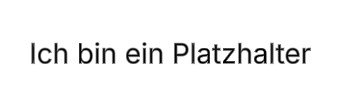
\includegraphics[width=0.5\linewidth]{inhalt/bilder/Platzhalter.jpg}
% 	\caption{}
% 	\label{fig:esp32_wordclock}
% \end{figure}

% Ein weiteres Segment bilden günstige Massenmarktprodukte, die über Onlineplattformen wie Alibaba oder vergleichbare Anbieter vertrieben werden~\cite{alibaba_wordclock}. 
% Diese Produkte liegen preislich meist im Bereich von etwa 10 € bis 150 € und zeichnen sich durch eine einfache technische Umsetzung sowie eine stark reduzierte Funktionalität aus. 
% Sie sind primär als dekorative Produkte einzuordnen und weisen sowohl in Bezug auf Materialqualität als auch Funktionsumfang deutliche Einschränkungen auf.

% \begin{figure}[H]
% 	\centering
% 	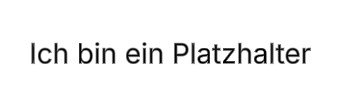
\includegraphics[width=0.5\linewidth]{inhalt/bilder/Platzhalter.jpg}
% 	\caption{}
% 	\label{fig:alibaba_wordclock}
% \end{figure}

% Die Untersuchung erfolgt anhand definierter Bewertungskriterien. 
% Neben funktionalen Eigenschaften werden der Kaufpreis sowie gestalterische Merkmale analysiert. 
% Hierzu zählen insbesondere Materialwahl, Lichtcharakteristik, Formfaktor und Integrationsfähigkeit in Wohnumgebungen. 
% Ein weiteres Kriterium stellt die zeitliche Präzision dar. 
% Dabei werden eingesetzte Zeitquellen, wie quarzbasierte Echtzeituhrmodule oder netzwerkbasierte Zeitsynchronisation, berücksichtigt. 

% Die systematische Gegenüberstellung ermöglicht die Identifikation von Gemeinsamkeiten und Unterschieden zwischen den betrachteten Systemen. 
% Auf dieser Grundlage lassen sich funktionale Defizite sowie Potenziale für innovative Erweiterungen ableiten. 
% Die gewonnenen Erkenntnisse fließen in die Konzeptionierung der im Rahmen dieser Arbeit entwickelten Wortuhr ein. 
% Die Ergebnisse sind tabellarisch in Tabelle~\ref{tab:vergleich_wordclock_ohne_diy} dargestellt.

% Aus der Gegenüberstellung ergibt sich eine deutliche Diskrepanz zwischen Designqualität und funktionaler Leistungsfähigkeit. 
% Insbesondere im Premiumsegment zeigt sich trotz hoher Preise ein eingeschränkter Funktionsumfang. 
% Systeme im mittleren Preissegment bieten erste Ansätze technischer Erweiterungen, erreichen jedoch keine umfassende funktionale Integration moderner Informationssysteme. 
% DIY-Systeme weisen hingegen eine hohe Funktionalität und Flexibilität bei vergleichsweise geringen Kosten auf, erfüllen jedoch häufig nicht die gestalterischen und konstruktiven Anforderungen eines marktfähigen Produkts.
% % Aus dieser Gegenüberstellung ergibt sich eine deutliche Diskrepanz zwischen Designqualität und funktionaler Leistungsfähigkeit. 
% % Die Tabelle 1 verdeutlicht, dass insbesondere im Premiumsegment trotz hoher Preise ein sehr eingeschränkter Funktionsumfang vorliegt. 
% % Systeme im mittleren Preissegment bieten erste Ansätze technischer Erweiterung, erreichen jedoch nicht die Tiefe funktionaler Integration moderner Informationssysteme. 
% % DIY-Systeme hingegen bieten ein hohes Maß an Funktionalität und Flexibilität bei vergleichsweise niedrigen Kosten, erreichen jedoch meist nicht die gestalterische und konstruktive Qualität eines marktfähigen Produkts.

% \begin{table}[h]
% \centering
% \begin{tabular}{|p{4cm}|p{3.5cm}|p{3.5cm}|p{3.5cm}|}
% \hline
% \textbf{Kriterium} & \textbf{Premium (z.\,B. QLOCKTWO / Biegert \& Funk)} & \textbf{Mittleres Segment (z.\,B. Build-Yours / Jupiter)} & \textbf{Massenmarkt (z.\,B. Alibaba)} \\
% \hline
% Preisbereich & ca. 1.500 € – 3.000 € & ca. 200 € – 600 € & ca. 10 € – 150 € \\
% \hline
% Zielsetzung & Designobjekt / Lifestyle & Kombination aus Technik \& Design & Dekorationsprodukt \\
% \hline
% Wortbasierte Zeitanzeige & o & o & o \\
% \hline
% Materialqualität & Sehr hoch (Metall, Holz) & Mittel bis hoch & Niedrig \\
% \hline
% Designfokus & Sehr hoch & Mittel & Gering \\
% \hline
% WLAN / Internet & x & o & x \\
% \hline
% App-Steuerung & x & o & x \\
% \hline
% Farb- / Anzeigeanpassung & x / sehr begrenzt & o & o (begrenzt) \\
% \hline
% Sekundenanzeige & o (teilweise) & x & x \\
% \hline
% Wetterdaten & x & x & x \\
% \hline
% Temperaturanzeige & x & x & x \\
% \hline
% Mondzeiten / Zusatzinfos & x & x & x \\
% \hline
% Erweiterbarkeit (APIs) & x & x & x \\
% \hline
% Benutzerfreundlichkeit & Sehr hoch & Hoch & Mittel \\
% \hline
% Produktreife & Sehr hoch & Hoch & Mittel \\
% \hline
% \end{tabular}
% \caption{Vergleich verschiedener Wortuhren in verschiedenen Preissegmenten.}
% \label{tab:vergleich_wordclock_ohne_diy}
% \end{table}

% %%%%%%%%%%%%%%%%%%%%%%%%%%%%%Tabelle mit ESP/DIY
% % \begin{table}[h]
% % \centering
% % \begin{tabular}{|p{4cm}|p{3cm}|p{3cm}|p{3cm}|p{3cm}|}
% % \hline
% % \textbf{Kriterium} & \textbf{Premium (z.\,B. QLOCKTWO / Biegert \& Funk)} & \textbf{Mittleres Segment (z.\,B. Build-Yours / Jupiter)} & \textbf{DIY / Maker (ESP32)} & \textbf{Massenmarkt (z.\,B. Alibaba)} \\
% % \hline
% % Preisbereich & ca. 1.500 € – 3.000 € & ca. 200 € – 600 € & ca. 50 € – 200 € & ca. 10 € – 150 € \\
% % \hline
% % Zielsetzung & Designobjekt / Lifestyle & Kombination aus Technik \& Design & Technische Plattform & Dekorationsprodukt \\
% % \hline
% % Wortbasierte Zeitanzeige & o & o & o & o \\
% % \hline
% % Materialqualität & Sehr hoch (Metall, Holz) & Mittel bis hoch & Variabel & Niedrig \\
% % \hline
% % Designfokus & Sehr hoch & Mittel & Gering & Gering \\
% % \hline
% % WLAN / Internet & x & o & o & x \\
% % \hline
% % App-Steuerung & x & o & o (optional) & x \\
% % \hline
% % Farb- / Anzeigeanpassung & x / sehr begrenzt & o & o & o (begrenzt) \\
% % \hline
% % Sekundenanzeige & o (teilweise) & x & o & x \\
% % \hline
% % Wetterdaten & x & x & o & x \\
% % \hline
% % Temperaturanzeige & x & x & o & x \\
% % \hline
% % Mondzeiten / Zusatzinfos & x & x & o & x \\
% % \hline
% % Erweiterbarkeit (APIs) & x & x & o & x \\
% % \hline
% % Benutzerfreundlichkeit & Sehr hoch & Hoch & Mittel & Mittel \\
% % \hline
% % Produktreife & Sehr hoch & Hoch & Niedrig & Mittel \\
% % \hline
% % \end{tabular}
% % \caption{Vergleich verschiedener WordClock-Segmente}
% % \label{tab:vergleich_wordclock}
% % \end{table}

% Vor diesem Hintergrund gewinnt die Entwicklung einer eigenen Wortuhr besondere Relevanz. 
% Ziel ist es, die bestehenden Schwächen der aktuellen Marktsegmente zu überwinden, indem eine Lösung geschaffen wird, die sowohl gestalterische als auch funktionale Anforderungen vereint. 
% Die entwickelte Wortuhr integriert neben der klassischen wortbasierten Zeitanzeige zusätzliche Funktionen wie Sekundenanzeige, Wetterdaten, Temperaturinformationen und Mondzeiten. 
% Durch den Einsatz eines internetfähigen Mikrocontrollers wird zudem die Grundlage für eine erweiterbare und zukunftsfähige Systemarchitektur geschaffen.

% Die Bewertung in der unterstehenden Tabelle~\ref{tab:bewertung_wordclock} zeigt, dass bestehende Systeme entweder in einzelnen Kategorien sehr stark sind, jedoch keine ganzheitlich ausgewogene Lösung darstellen. 
% Premiumprodukte erreichen hohe Werte im Bereich Design und Benutzerfreundlichkeit, schneiden jedoch im Funktionsumfang und in der Erweiterbarkeit schwach ab. 
% DIY-Systeme hingegen überzeugen durch hohe Funktionalität und Erweiterbarkeit, weisen jedoch Defizite im Design und in der Benutzerfreundlichkeit auf. 
% Die entwickelte Wortuhr erreicht hingegen in allen Kategorien hohe Bewertungen und stellt somit eine ausgewogene und leistungsfähige Gesamtlösung dar.

% \begin{table}[h]
% \centering
% \begin{tabular}{|c|c|c|c|c|c|c|}
% \hline
% \textbf{Produkt} & \textbf{Design} & \textbf{Funktion} & \textbf{Usability} & \textbf{Erweiterbarkeit} & \textbf{Preis-Leistung} & \textbf{Gesamt} \\
% \hline
% QLOCKTWO & 5 & 2 & 5 & 1 & 2 & 3,05 \\
% \hline
% Jupiter & 3 & 3 & 4 & 2 & 3 & 3,05 \\
% \hline
% Massenmarkt & 2 & 1 & 3 & 1 & 4 & 2,10 \\
% \hline
% Eigene Wortuhr & 4 & 5 & 4 & 5 & 4 & 4,45 \\
% \hline
% \end{tabular}
% \caption{Bewertung verschiedener WordClock-Konzepte}
% \label{tab:bewertung_wordclock}
% \end{table} \todo{Tabelle überarbeiten und page matching}

% %%%%%%%%%%%%%%%%%%%Tabelle mit ESP/DIY
% % \begin{table}[h]
% % \centering
% % \begin{tabular}{|c|c|c|c|c|c|c|}
% % \hline
% % \textbf{Produkt} & \textbf{Design} & \textbf{Funktion} & \textbf{Usability} & \textbf{Erweiterbarkeit} & \textbf{Preis-Leistung} & \textbf{Gesamt} \\
% % \hline
% % QLOCKTWO & 5 & 2 & 5 & 1 & 2 & 3,05 \\
% % \hline
% % Jupiter & 3 & 3 & 4 & 2 & 3 & 3,05 \\
% % \hline
% % DIY (ESP32) & 2 & 5 & 2 & 5 & 5 & 3,70 \\
% % \hline
% % Massenmarkt & 2 & 1 & 3 & 1 & 4 & 2,10 \\
% % \hline
% % Eigene Wortuhr & 4 & 5 & 4 & 5 & 4 & 4,45 \\
% % \hline
% % \end{tabular}
% % \caption{Bewertung verschiedener WordClock-Konzepte}
% % \label{tab:bewertung_wordclock}
% % \end{table}

% Damit positioniert sich die entwickelte Lösung zwischen den bestehenden Marktsegmenten und adressiert gezielt eine bislang nur unzureichend besetzte Nische. 
% Sie stellt nicht nur eine technische Erweiterung bestehender Systeme dar, sondern verfolgt den Ansatz, die Wortuhr von einem reinen Designobjekt zu einem intelligenten Informationssystem weiterzuentwickeln. 
% Diese Kombination aus ästhetischer Gestaltung und funktionaler Erweiterbarkeit begründet die Relevanz der eigenen Entwicklung sowohl aus technischer als auch aus marktbezogener Perspektive.


% % Im Fokus stehen dabei vier kommerziell vertrieben Wortuhren unterschiedlicher Hersteller:innen und Preissegmente. 
% % Die Untersuchten Wortuhren sind in Abbildung~\ref{fig:VergleichWortuhren} dargestellt.
% % \begin{figure}[H]
% %     \centering
% %     \begin{subfigure}[t]{0.35\textwidth}
% %         \centering
% %         
\includegraphics[width=\linewidth]{inhalt/bilder/QlockTwoDessert.png}
% %         \caption{Das Model Earth 45 von QlockTwo mit deutschem Text im Design Dessert~\cite{QlockTwoDesert}.}
% % 	    \label{fig:QlockTwoDessert}
% %     \end{subfigure}
% %     \hfill
% %     \begin{subfigure}[t]{0.35\textwidth}
% %         \centering
% %         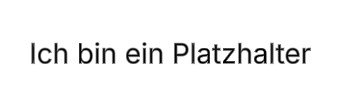
\includegraphics[width=\linewidth]{inhalt/bilder/Platzhalter.jpg}
% %         \caption{rechts oben.}
% %         \label{fig:sub1_b}
% %     \end{subfigure}
% %     \vspace{0.8em}
% %     \begin{subfigure}[t]{0.35\textwidth}
% %         \centering
% %         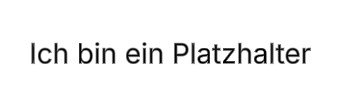
\includegraphics[width=\linewidth]{inhalt/bilder/Platzhalter.jpg}
% %         \caption{links unten.}
% %         \label{fig:sub1_c}
% %     \end{subfigure}
% %     \hfill
% %     \begin{subfigure}[t]{0.35\textwidth}
% %         \centering
% %         
\includegraphics[width=\linewidth]{inhalt/bilder/QlockTwoDessert.png}
% %         \caption{rechts unten.}
% %         \label{fig:sub1_d}
% %     \end{subfigure}
% %     \caption{Vergleich von vier kommerziell vertriebenen Wortuhren verschiedener Hersteller:innen.}
% %     \label{fig:VergleichWortuhren}
% % \end{figure}

% % Abbildung~\ref{fig:QlockTwoDessert} zeigt das Model Earth 45 des Herstellers Qlocktwo im Design Desert in deutscher Sprache.
% % % Hier text welche 4 und warum, darunter bild mit 4 subfigures je eine Uhr.
% % Diese Produkte repräsentieren verschiedene Marktsegmente hinsichtlich Kosten, Funktionsumfang und technischer Ausführung. 

% % Die Untersuchung erfolgt anhand selbst definierter Bewertungskriterien. 
% % Neben funktionale Eigenschaften werden auch der Kaufpreis und gestalterische Merkmale analysiert. 
% % Darunter Materialwahl, Lichtcharakteristik, Formfaktor und Integrationsmöglichkeiten in Wohnumgebungen. 
% % Ein weiteres Kriterium stellt die zeitliche Präzision dar. 
% % Hierbei werden eingesetzte Zeitquellen, beispielsweise quarzbasierte Echtzeituhrmodule oder netzwerkbasierte Zeitsynchronisation, betrachtet. 

% % Die Gegenüberstellung ermöglicht die Identifikation von Gemeinsamkeiten und Unterschieden zwischen den betrachteten Systemen. 
% % Auf dieser Basis lassen sich funktionale Defizite sowie Potenziale für innovative Erweiterungen ableiten. 
% % Die gewonnenen Erkenntnisse fließen in die Konzeptionierung der im Rahmen dieser Arbeit entwickelten Wortuhr ein.
% % Die Ergebnisse sind Tabellarisch in Tabelle~\ref{tab:VergleichWortuhren} dargestellt.
    % \section{Relevanz des Projekts} \todo{Gegenlesen}
Vor diesem Hintergrund gewinnt die Entwicklung einer eigenen Wortuhr besondere Relevanz. 
Ziel ist es, bestehende Schwächen der aktuellen Marktsegmente gezielt zu adressieren und eine Lösung zu entwickeln, die gestalterische und funktionale Anforderungen integriert. 
Die entwickelte Wortuhr soll folgenden, grundlegenden und zusätzliche Funktionen aufweisen und darstellen:

\begin{enumerate}
	\item Kontinuierliche und unterbrechungsfreie wortbasierte Zeitanzeige von Stunde, Minute und Sekunde
	\item Wortbasierte Anzeige der Außentemperatur auf Basis definierter Schwellenwerte
	\item Wortbasierte Darstellung von Wetterinformationen
	\item Symbolische Darstellung der Tageszeit
	\item Symbolische Darstellung der Mondphase
	\item Symbolische Darstellung der Raumfeuchtigkeit
	\item Symbolische Darstellung der Innenraumtemperatur
\end{enumerate}

Die Bewertung in Tabelle~\ref{tab:bewertung_wordclock} zeigt, dass bestehende Systeme entweder in einzelnen Kategorien hohe Ausprägungen erreichen oder deutliche Defizite aufweisen, jedoch keine ausgewogene Gesamtlösung darstellen. 
Premiumprodukte erzielen hohe Werte im Bereich Design und Benutzerfreundlichkeit, weisen jedoch Defizite im Funktionsumfang und in der Erweiterbarkeit auf. 
DIY-Systeme hingegen bieten eine hohe Funktionalität und Erweiterbarkeit, erfüllen jedoch häufig nicht die Anforderungen an Design und Benutzerfreundlichkeit. 

\begin{table}[h]
\centering
\begin{tabular}{|c|c|c|c|c|c|c|}
\hline
\textbf{Produkt} & \textbf{Design} & \textbf{Funktion} & \textbf{Usability} & \textbf{Erweiterbarkeit} & \textbf{Preis-Leistung} & \textbf{Gesamt} \\
\hline
QLOCKTWO & 5 & 2 & 5 & 1 & 2 & 3,05 \\
\hline
Jupiter & 3 & 3 & 4 & 2 & 3 & 3,05 \\
\hline
Massenmarkt & 2 & 1 & 3 & 1 & 4 & 2,10 \\
\hline
Eigene Wortuhr & 4 & 5 & 4 & 5 & 4 & 4,45 \\
\hline
\end{tabular}
\caption{Bewertung verschiedener WordClock-Konzepte}
\label{tab:bewertung_wordclock}
\end{table} \todo{Tabelle überarbeiten und page matching}

Vor diesem Hintergrund wird im Rahmen dieser Arbeit das Ziel verfolgt, eine Wortuhr zu entwickeln, die in allen betrachteten Kategorien hohe Bewertungen erreicht. 
Hierdurch soll eine ausgewogene und leistungsfähige Gesamtlösung realisiert werden.
Damit positioniert sich die entwickelte Lösung zwischen den bestehenden Marktsegmenten und adressiert eine bislang nur unzureichend besetzte Nische. 
Sie stellt nicht nur eine technische Erweiterung bestehender Systeme dar, sondern verfolgt den Ansatz, die Wortuhr von einem Designobjekt zu einem Informationssystem weiterzuentwickeln. 
Die Kombination aus gestalterischer Qualität und funktionaler Erweiterbarkeit begründet die Relevanz der eigenen Entwicklung sowohl aus technischer als auch aus marktbezogener Perspektive.

    
%   _________Kapitel 2_________
\chapter{Stand der Technik und Grundlagen}
    \section{Grundlegendes Funktionsprinzip von Wortuhren}
Eine Wortuhr stellt die aktuelle Zeit nicht numerisch, sondern durch hervorgehobene Wörter in natürlicher Sprache dar. 
Hierzu wird ein fest definiertes Wortfeld verwendet, in dem durch gezielte Aktivierung einzelner Buchstaben eine lesbare Zeitangabe entsteht.
Diese sind in einer Matrix angeordnet und bilden verschiedene, teilweise überlappende Wörter. 
Die Darstellung erfolgt durch gezielte Beleuchtung einzelner Buchstaben mittels einer hinterlegten Lichtquelle.

Die Zeit wird durch eine Referenzquelle bereitgestellt und in einer Logikeinheit numerisch verarbeitet. 
Anschließend erfolgt eine regelbasierte Umwandlung in sprachliche Ausdrücke.
Dies wird als im folgenden als Wordmapping bezeichnet. 
Die Zuordnung der Zeitwerte zu den darzustellenden Wörtern ist softwareseitig definiert und wird durch ein geeignetes Logikmodul umgesetzt. 
Dabei kommen typische Formulierungen wie „nach“, „vor“ oder „halb“ zum Einsatz. 
Die Anzeige basiert auf diskreten Zeitintervallen, deren Auflösung die Struktur und Größe der Wortmatrix bestimmt.

Bei der sprachlichen Zeitdarstellung sind mehrere Sonderfälle zu berücksichtigen. 
Hierzu zählt die korrekte Behandlung der Stunde bei „ein Uhr“ im Vergleich zur Verwendung von „eins“ in anderen Kontexten, beispielsweise „halb eins“. 
Weiterhin ist der Übergang zwischen zwei Stunden zu beachten, insbesondere bei Formulierungen wie „vor“ und „halb“, bei denen bereits auf die folgende Stunde Bezug genommen wird.

Zusätzlich erfordern die Zeitpunkte 0:00 Uhr und 12:00 Uhr eine eindeutige Definition. 
Auch Randbereiche zwischen zwei Intervallen, beispielsweise kurz vor oder nach einem Fünf-Minuten-Schritt, müssen eindeutig zugeordnet werden, um eine konsistente Anzeige sicherzustellen.
% Eine Wortuhr stellt die aktuelle Zeit nicht numerisch, sondern durch hervorgehobene Wörter in natürlicher Sprache dar. 
% Hierzu wird ein fest definiertes Wortfeld verwendet, in dem durch gezielte Aktivierung einzelner Buchstaben eine lesbare Zeitangabe entsteht.
% Die Buchstaben sind in einer Matrix angeordnet und bilden verschiedene, teilweise überlappende Wörter. 
% Die Darstellung erfolgt durch Beleuchtung der zugehörigen Buchstaben mittels einer hinterlegten Lichtquelle, welche  je einen Buchstaben beleuchtet.

% Die Zeit muss durch eine entsprechende Referenzquelle zur Verfügung gestellt werden.
% Sie wird mit einer Logikeinheit numerisch verarbeitet und regelbasiert in sprachliche Ausdrücke überführt. 
% Die Regeln, wann welche Buchstaben gesetzt werden, müssen Softwareseitig programmiert sein und auf einem geeigneten Logikmodul prozessiert werden.
% Dabei werden typische Formulierungen wie „nach“, „vor“ oder „halb“ verwendet. 
% Die Anzeige basiert auf diskreten Zeitintervallen, was abhängig der Zeitlichen Genauigkeit die Struktur und Größe der Wortmatrix bestimmt.

% Bei der sprachlichen Zeitdarstellung sind mehrere Sonderfälle zu berücksichtigen. 
% Hierzu zählt die korrekte Behandlung der Stunde bei „ein Uhr“ im Vergleich zur Verwendung von „eins“ in anderen Kontexten, z.B. „Es ist halb eins“. 
% Weiterhin ist der Übergang zwischen zwei Stunden zu beachten, insbesondere bei Formulierungen wie „vor“ und „halb“, bei denen bereits auf die folgende Stunde Bezug genommen wird. 

% Zusätzlich erfordern die Zeitpunkte 0:00 und 12:00 eine eindeutige Definition, da diese sowohl als Beginn eines neuen Tages als auch als Abschluss eines Zeitraums interpretiert werden können. 
% Auch Randbereiche zwischen zwei Intervallen, beispielsweise kurz vor oder nach einem Fünf-Minuten-Schritt, müssen eindeutig zugeordnet werden, um eine konsistente Anzeige sicherzustellen.
    \section{Zeitdarstellung in natürlicher Sprache} \todo{text}
Sprachliche Zeitlogik
Besonderheiten im Deutschen
Einfluss auf Anzeige und Logik
Wichtig für spätere Software-Logik
    % ===========Für anderes Kapitel eventuell verwenden
% Für die Anzeige der Wortuhr werden adressierbare RGB-Leuchtdioden (LEDs) vom Typ WS2812B eingesetzt. 
% Diese ermöglichen eine individuelle Ansteuerung 
% jeder einzelnen LED innerhalb eines Verbunds. Die LEDs sind dabei physikalisch in Reihe 
% geschaltet (Daisy-Chain) und werden über eine einzige serielle Datenleitung gesteuert. 
% Jede LED verfügt über einen integrierten Controller, der die eingehenden Datenpakete 
% verarbeitet, den für sich bestimmten Anteil extrahiert und das verbleibende Signal für 
% die nachfolgenden LEDs aufbereitet und weiterleitet~\cite{Worldsemi2013}. 

\section{WS2812B LEDs als Anzeigeelement}
Die WS2812B ist eine integrierte RGB-Leuchtdiode mit eingebauter Steuerelektronik. 
Sie kombiniert eine Lichtquelle und eine digitale Ansteuerlogik in einem gemeinsamen Gehäuse der Bauform 5050. 
Dadurch entfällt die Notwendigkeit externer Treiberschaltungen für einzelne LEDs, was den Schaltungsaufwand reduziert und die Integration vereinfacht~\cite{Worldsemi2013}.

Ein wesentliches Merkmal der WS2812B ist die serielle Ansteuerung über eine einzelne Datenleitung. 
Die Kommunikation erfolgt über ein digitales Protokoll, bei dem die Daten bitweise übertragen werden. 
Jede LED empfängt dabei einen Datenstrom, verarbeitet die ersten 24 Bit zur eigenen Darstellung und leitet die verbleibenden Daten an nachfolgende LEDs weiter. 
Dieses Prinzip ermöglicht die Realisierung langer LED-Ketten mit minimalem Verdrahtungsaufwand~\cite{Worldsemi2013}. 

Die Farbdarstellung basiert auf drei integrierten Leuchtdioden für die Grundfarben Rot, Grün und Blau. 
Für jede dieser Komponenten stehen 8 Bit zur Verfügung, wodurch sich insgesamt 24 Bit pro LED ergeben. 
Dies ermöglicht die Darstellung von bis zu 16.777.216 verschiedenen Farbwerten. 
Die Datenübertragung erfolgt in einer fest definierten Reihenfolge der Farbkanäle, wodurch eine konsistente Farbwiedergabe gewährleistet wird.
Die Versorgung der WS2812B erfolgt mit +5V. 
Jede LED enthält eine interne Konstantstromsteuerung, wodurch eine gleichmäßige Helligkeit unabhängig von Versorgungsschwankungen erreicht wird~\cite{Worldsemi2013}. 

Ein weiterer Vorteil liegt in der Möglichkeit zur einfachen Kaskadierung (vgl. Abb.~\ref{fig:KaskadeLED}).
Mehrere LEDs können direkt hintereinander geschaltet werden, wobei der Ausgang einer LED mit dem Eingang der nächsten verbunden wird. 
Die maximale Anzahl der kaskadierbaren LEDs hängt primär von der Datenrate und der gewünschten Aktualisierungsfrequenz ab. 
Bei typischen Anwendungen können mehrere hundert bis über 1000 LEDs ohne zusätzliche Signalverstärkung betrieben werden~\cite{Worldsemi2013}.

\begin{figure}[H]
	\centering
	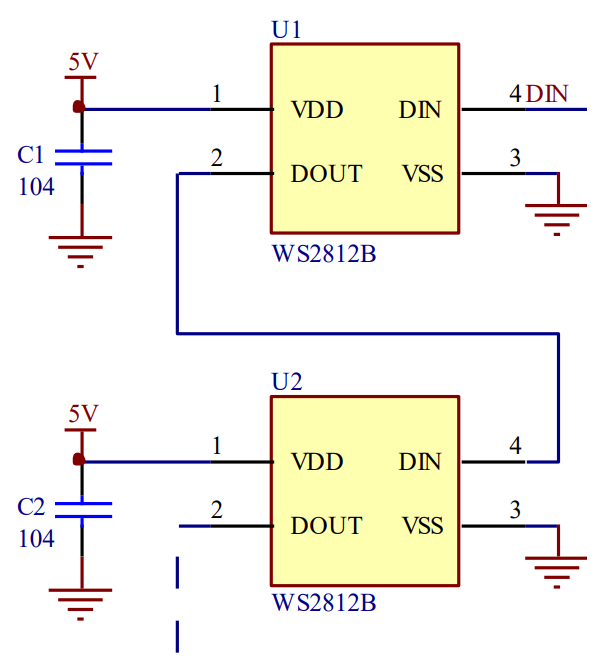
\includegraphics[width=0.5\linewidth]{inhalt/bilder/KaskadeLED.png}
	\caption{Schaltbild zur Kaskadierung von WS2812B LEDs mit einer Versorgungsspannung von +5V. Mit VDD als Versorgungsspannung, DIN als Datensignal Eingang, DOUT als Datensignal Ausgang und VSS als als Ground~\cite{Worldsemi2013}.}
	\label{fig:KaskadeLED}
\end{figure}

Für Anwendungen wie Wortuhren ergibt sich aus diesen Eigenschaften eine geeignete Architektur. 
Die einzelne Adressierbarkeit ermöglicht die gezielte Darstellung wobei die geringe Anzahl benötigter Steuerleitungen in einem geringen Verdrahtungsaufwand resultiert. 
Gleichzeitig erlaubt die hohe Farbauflösung eine flexible Gestaltung der Anzeige, beispielsweise zur Differenzierung von Funktionen oder Zuständen~\cite{Worldsemi2013}.

% LED-Typen (RGB, adressierbar)
% Ansteuerungsprinzipien
% Vor- und Nachteile
% RGB-LEDs
% Adressierbare LEDs (z. B. WS2812, SK6812)
% LED-Matrix
% LED-Streifen
% PWM-Helligkeitssteuerung
% Farbtemperatur
% Gleichmäßige Ausleuchtung
% Diffusoren (Acryl, Milchglas)
% Lichtkammern / Trennstege
% Hot-Spot-Vermeidung
% Energieeffizienz von LEDs

% adressierbare RGB-LEDs, NeoPixel/WS2812-Prinzip, Datenleitung, RGB-Farbmischung, Helligkeitssteuerung, LED-Matrix, separater Sekundenring
% adressierbare LEDs (WS2812 / NeoPixel)
% serielle Datenübertragung (1-Draht-Protokoll)
% RGB-Farbmodell (additive Farbmischung)
% Helligkeitssteuerung (PWM / softwareseitige Skalierung)
% Verkettung mehrerer LEDs (Daisy Chain)
% Timing-Anforderungen
% Energiebedarf pro LED
% Matrix vs. Streifen
% separater Sekundenring als Zusatzanzeige
    \input{inhalt/textkapitel/Kapitel 2/235_Entwicklung von Steuerungs- und Eingebetteten Systemen.tex}
    \section{Mikrocontrollerbasierte Steuerung} \todo{text}
% Mikrocontroller
% Embedded Systems
% Echtzeitfähigkeit
% Ressourcenbeschränkungen
% Task-Scheduling
% Energiemanagement
% Firmware-Updates
% ESP32 als Mikrocontroller, zyklische Hauptschleife, nicht-blockierende Aktualisierung mit millis(), globale Zustände, Zustandsvariablen, Trennung in Funktionsgruppen

        \subsection{ESP32 als zentrale Steuereinheit} \todo{text}
% ESP32 als SoC (CPU, WLAN, GPIO)
% Echtzeitfähigkeit (bedingt)
% Energieeffizienz
% GPIO-Pins zur LED-Ansteuerung
% integriertes WLAN-Modul
% Speicher (RAM/Flash)
% Arduino-Framework

% Als zentrale Steuereinheit wird ein Mikrocontroller der ESP32-Familie eingesetzt. Dieser integriert neben der Recheneinheit auch Kommunikationsschnittstellen wie WLAN sowie verschiedene Ein- und Ausgänge. Dadurch eignet er sich besonders für eingebettete Anwendungen mit Netzwerkfunktionalität. Die Ansteuerung der LEDs erfolgt über digitale GPIO-Pins, während gleichzeitig Netzwerkkommunikation und Zeitverarbeitung durchgeführt werden können.
        \subsection{Zeitsynchronisation über NTP}
Eine zuverlässige Zeitbasis ist für zeitabhängige Systeme erforderlich, da lokale Uhren ohne externe Synchronisation Abweichungen aufweisen können.
Mills beschreibt, dass lokale Uhren häufig auf Quarzoszillatoren basieren, deren Abweichung bis zu etwa einer Sekunde pro Tag betragen kann~\cite{mills1991ntp}.

Das \gls{ntp}, dient zur Verteilung von Zeitinformationen in verteilten Netzwerken~\cite{mills1991ntp}.
Das Protokoll nutzt eine hierarchische Struktur aus primären und sekundären Zeitservern.
Primäre Zeitserver sind direkt mit einer Referenzzeitquelle verbunden.
Sekundäre Zeitserver beziehen ihre Zeit über Netzwerkpfade von primären oder weiteren sekundären Servern.
Die Synchronisation erfolgt über den Austausch von Zeitstempeln zwischen den beteiligten Systemen.
Aus diesen Zeitstempeln werden die Übertragungsverzögerung und die Zeitabweichung zwischen lokaler Uhr und Zeitserver bestimmt~\cite{mills1991ntp}.
Auf dieser Grundlage kann die lokale Uhr korrigiert werden.

Für den Einsatz in Netzwerken berücksichtigt \gls{ntp} schwankende Übertragungsverzögerungen und mögliche Störungen.
Dazu werden Filter-, Auswahl- und Kombinationsverfahren verwendet, um geeignete Zeitinformationen auszuwählen.
Nach Mills kann mit \gls{ntp} in weiten Teilen des Internets eine Zeitgenauigkeit im Bereich weniger Millisekunden erreicht werden~\cite{mills1991ntp}.
Für die entwickelte Wortuhr ist diese Genauigkeit ausreichend, da die Zeitanzeige in diskreten Minutenintervallen erfolgt.
\gls{ntp} stellt damit eine geeignete Grundlage dar, um die interne Zeitbasis des Mikrocontrollers regelmäßig mit einer externen Referenzzeit abzugleichen.
% Network Time Protocol (NTP)
% UTC vs. lokale Zeit
% Zeitzonen und Sommerzeit (DST)
% Zeitserver (pool.ntp.org)
% Synchronisationsstrategien (Start + regelmäßig)
% Fehlerfälle (Timeout, Retry)
% Driftkorrektur
        %\subsection{Zyklische Programmlogik und Zustandssteuerung}\todo{3.5.3 notwendig?--> Checken}

    \section{Netzwerkbasierte Bedien- und Schnittstellenkonzepte} \todo{text}
        \subsection{WLAN-Anbindung eingebetteter Systeme} \todo{text}
% WLAN-Modus (Station Mode)
% IP-Adresse (DHCP)
% Verbindungsaufbau
% Netzwerkabhängigkeit
% lokale vs. Cloud-Systeme

% Die Einbindung des Systems in ein lokales Netzwerk erfolgt über die integrierte WLAN-Schnittstelle des Mikrocontrollers. Nach dem Verbindungsaufbau erhält das Gerät automatisch eine IP-Adresse und kann über diese im Netzwerk angesprochen werden. Dadurch wird eine direkte Kommunikation zwischen Nutzer und Gerät ohne zusätzliche Infrastruktur ermöglicht.
        \subsection{HTTP-Webserver und lokale Browsersteuerung} \todo{text}
% HTTP-Protokoll
% Client-Server-Prinzip
% Embedded Webserver
% GET-Requests
% URL-Parameter
% HTML-Generierung im Mikrocontroller
% einfache Webinterfaces

% Zur Bedienung der Wortuhr wird ein integrierter HTTP-Webserver verwendet. Dieser stellt eine HTML-basierte Benutzeroberfläche bereit, die über einen Webbrowser aufgerufen werden kann. Steuerbefehle werden dabei über HTTP-Anfragen übertragen und direkt vom Mikrocontroller verarbeitet. Dadurch ist keine zusätzliche Softwareinstallation erforderlich.
        \subsection{JSON-Schnittstellen für Statusdaten}
\gls{json} wird als Datenformat zur Übertragung von Zustandsinformationen eingesetzt.
Es handelt sich um ein standardisiertes, menschenlesbares Format, das unabhängig von der verwendeten Programmiersprache genutzt werden kann~\cite{wehner_json_iot}.
Dadurch eignet es sich für den Austausch von Daten zwischen unterschiedlichen Systemen und Komponenten.

Aufgrund seiner einfachen und kompakten Struktur verursacht \gls{json} nur geringen Kommunikationsaufwand.
Dies ist insbesondere in eingebetteten Systemen mit begrenzten Ressourcen von Vorteil, da unnötiger Overhead vermieden wird~\cite{wehner_json_iot}.
Durch die einfache Parsbarkeit und die geringe Komplexität eignet sich das \gls{json}-Format zudem für den Einsatz in heterogenen und verteilten Systemen~\cite{wehner_json_iot}.
Damit wird eine Grundlage geschaffen, um die Wortuhr in übergeordnete Systeme einzubinden oder Statusinformationen automatisiert auszuwerten.

% Vielleicht späteres Kapitel
% In der Studienarbeit wird das \gls{json}-Format zur Bereitstellung maschinenlesbarer Statusdaten verwendet.
% Dazu gehören unter anderem Informationen zum Betriebszustand, zur Uhrzeit, zu Sensorwerten sowie zu Konfigurationsparametern.
% Die strukturierte Darstellung ermöglicht eine einfache Weiterverarbeitung der Daten durch externe Systeme.

% JSON als Datenformat
% REST-ähnliche APIs
% maschinenlesbare Daten
% Debugging
% Integration in andere Systeme möglich
    \input{inhalt/textkapitel/Kapitel 2/260_Datenquellen und externe Schnittstellen.tex}
        \input{inhalt/textkapitel/Kapitel 2/261_Sensordaten in IoT-Systemen.tex}
        \subsection{Open-Meteo als externe Wetterdatenquelle}
Eine häufig genutzte Quelle für Wetterdaten ist die Open-Meteo-API, welche als frei zugängliche und quelloffene Web-\gls{api} zur Bereitstellung meteorologischer Informationen dient. 
Sie ermöglicht den Zugriff auf Wetterdaten ohne Authentifizierung und eignet sich insbesondere für nicht-kommerzielle Anwendungen~\cite{openmeteo}.

Die \gls{api} basiert auf dem \gls{http}-Protokoll und liefert die angeforderten Daten in einem strukturierten \gls{json}-Format. 
Dadurch wird eine einfache Integration in eingebettete Systeme sowie in verschiedene Programmiersprachen ermöglicht. 
Die Anfrage erfolgt über eine \gls{url} mit spezifischen Parametern, beispielsweise zur Angabe von geografischer Breite und Länge. 
Die bereitgestellten Daten umfassen unter anderem Temperatur, Windgeschwindigkeit und Luftfeuchtigkeit, welche sowohl für aktuelle Zustände als auch in Form zeitlich aufgelöster Verlaufsdaten verfügbar sind~\cite{openmeteo}.

Die zugrunde liegenden Wetterinformationen basieren auf einer Kombination verschiedener Datenquellen, darunter Messungen von Satelliten, Radarsystemen sowie weiteren Sensornetzwerken~\cite{openmeteo}. 
Zur Gewährleistung einer hohen Aktualität werden die verwendeten Wettermodelle in kurzen Zeitintervallen aktualisiert.
Durch die standardisierte Bereitstellung über \gls{http} und \gls{json} sowie die kontinuierliche Aktualisierung der Daten stellt die Open-Meteo-\gls{api} eine geeignete Grundlage für die Integration externer Wetterinformationen für den vorliegenden Anwendungsfall dar~\cite{openmeteo}.

Die Kommunikation mit der API erfolgt über \gls{https}-basierte \gls{rest}-Schnittstellen. 
\gls{https} stellt die abgesicherte Variante des HTTP-Protokolls dar und basiert auf der Übertragung von HTTP über \gls{ssl} bzw. \gls{tls}. 
Dabei werden die Kommunikationspartner authentifiziert und die anschließende Datenübertragung vertraulich umgesetzt. 
Dies erhöht die Sicherheit der Kommunikation, kann jedoch zusätzliche Aufwände durch Handshake, Zertifikatsprüfung und kryptografische Operationen verursachen~\cite{naylor2014https}.

Eine \gls{rest}-Schnittstelle ist eine spezialisierte Form einer Programmierschnittstelle, die auf dem Architekturprinzip \gls{rest} basiert.
Sie ermöglicht die Kommunikation zwischen Client und Server über standardisierte HTTP-Methoden sowie eindeutig adressierbare Ressourcen.
Dabei erfolgt der Datenaustausch typischerweise zustandslos und unter Nutzung einheitlicher Schnittstellen, häufig im JSON-Format~\cite{RESTAPI}.
        \subsection{Verarbeitung und Nutzung der Wetterdaten}Allgemein ist die Integration externer Datenquellen mit Herausforderungen verbunden, insbesondere hinsichtlich Verfügbarkeit und Zuverlässigkeit der bereitgestellten Dienste~\cite{7123563}. 
Bei Ausfall der Verbindung oder des Dienstes können keine aktuellen Daten abgerufen werden. 
Daher ist eine geeignete Fehlerbehandlung erforderlich, um weiterhin einen stabilen Systembetrieb sicherzustellen.

Für die Darstellung der Wetterdaten wird eine vereinfachte Klassifikation der Messwerte verwendet. 
Kontinuierliche Größen wie die Temperatur werden in diskrete Bereiche unterteilt. 
Dadurch wird eine schwellwertabhängige Darstellung im Fall der Wortuhr ermöglicht. 
Beispielsweise können Temperaturbereiche in Kategorien wie kühl, frisch oder warm eingeteilt werden.

Neben der Temperatur können auch Wetterzustände wie ein klarer Himmel, Bewölkung oder Niederschlag berücksichtigt werden. 
Diese Zustände werden aus den bereitgestellten Daten abgeleitet und ebenfalls über Schwellenwerte klassifiziert. 
Dadurch wird eine schnelle Interpretation und Darstellung der aktuellen Wetterlage ermöglicht. 

Die Verarbeitung der Daten erfolgt zyklisch, wobei in definierten Zeitintervallen neue Wetterinformationen vom externen Dienst abgerufen werden. 
Zwischen den Aktualisierungen werden die zuletzt gültigen Werte weiterhin verwendet, um eine kontinuierliche Anzeige sicherzustellen.
Durch die Nutzung standardisierter Schnittstellen können Datenquellen einfach integriert und in bestehende Systeme eingebunden werden.

    %\section{Ambient Displays und Human-Computer Interaction} \todo{text}
% NEU: 2.7 Ambient Displays und HCI (Human-Computer Interaction)
% Dieses Kapitel verleiht deiner Arbeit ein sehr starkes wissenschaftliches Fundament. Nutze hierfür deine bereitgestellten wissenschaftlichen Paper:
% Grundlagen von Ambient Information Systems (AIS): Beschreibe Ambient Displays als Systeme, die nicht-kritische Informationen (wie das Wetter oder die Mondphase) kontinuierlich am Rand der menschlichen Wahrnehmung ("periphery of attention") darstellen
% . Im Gegensatz zu Smartphones oder Monitoren, die den vollen Fokus erfordern, können Ambient Displays "im Vorbeigehen" erfasst werden, ohne primäre Tätigkeiten zu unterbrechen
% .
% Calm Technology: Zitiere hier die extrem oft zitierten Pioniere Mark Weiser und John Seely Brown. Das Ziel von "Calm Computing" ist es, Technologie so zu gestalten, dass sie fließend zwischen dem Zentrum und der Peripherie unserer Aufmerksamkeit wechseln kann
% . Ein gutes Ambient Display informiert uns, ohne uns zu dominieren oder zu stressen
% .
% Praxisbeispiele in der HCI: Erwähne verwandte Forschungsansätze, bei denen Uhren als Ambient Displays genutzt wurden. Ein prominentes Beispiel aus der Literatur ist die Wherebouts Clock (die den Aufenthaltsort von Familienmitgliedern anzeigt) oder die Google Clock (die Termine durch farbliche Codierung im Hintergrund signalisiert)
% . Deine Wortuhr schlägt genau in diese Kerbe: Sie nutzt die Ästhetik eines Alltagsgegenstandes, um komplexe Smart-Home- und Wetterdaten unaufdringlich darzustellen
% .


% Für Kapitel 1.1: Motivation und Problemstellung
% (Hier begründen Sie die Relevanz Ihrer Arbeit über das Problem der Informationsüberflutung und den Lösungsansatz der "Calm Technology".)
% Textvorschlag:
% "In der heutigen Zeit sehen sich Nutzer durch die stetige Zunahme von vernetzten Geräten und Pervasive Computing mit einer wachsenden Informationsüberflutung (Information Overload) konfrontiert
% . Klassische Interfaces wie Smartphones oder PC-Bildschirme fordern meist die volle Aufmerksamkeit des Nutzers ein und reißen ihn aus seinem aktuellen Kontext heraus
% . Um dieser kognitiven Belastung entgegenzuwirken, forderten Mark Weiser und John Seely Brown bereits in den späten 1990er Jahren mit dem Paradigma der Calm Technology, dass Technologie nahtlos in den Hintergrund treten und Informationen unaufdringlich am Rande der Aufmerksamkeit – in der Peripherie – vermitteln sollte
% .
% Die Relevanz des vorliegenden Projekts liegt in der Anwendung genau dieses Prinzips auf den Smart-Home-Kontext. Während klassische Wortuhren primär ästhetischen Zwecken dienen und moderne Smart Displays häufig kognitiv überladen sind, zielt die hier entwickelte WordClock darauf ab, als sogenanntes Ambient Information System (AIS) zu fungieren
% . Durch die ästhetische, wortbasierte Anzeige relevanter Zusatzdaten (wie exakte Minuten, Wetter oder Mondphasen) wird eine Brücke zwischen Dekoration und multifunktionalem Smart-Home-Interface geschlagen
% . Die Informationen sind stets präsent, erfordern jedoch keine unmittelbare Interaktion und binden keine unnötigen kognitiven Ressourcen
% ."
% Für das NEUE Kapitel 2.2: Wissenschaftliches Umfeld: Ambient Displays und HCI
% (Hier schaffen Sie das theoretische Fundament und belegen, dass Ihr Ansatz state-of-the-art in der Forschung ist.)
% Textvorschlag:
% "Die konzeptionelle Basis für die erweiterte WordClock bilden Erkenntnisse aus dem Bereich der Mensch-Computer-Interaktion (HCI), speziell zu Ambient Information Systems und Peripheral Interaction.
% Ambient Information Systems (AIS) Ambient Information Systems präsentieren Informationen kontinuierlich und unaufdringlich im Hintergrund der menschlichen Wahrnehmung
% . Ihr Ziel ist es, den Nutzer über nicht-kritische Informationen (wie z. B. das Wetter) auf dem Laufenden zu halten, ohne ihn bei seinen primären Tätigkeiten zu stören
% . Diese Systeme nutzen die menschliche Fähigkeit zur präattentiven Verarbeitung, wodurch Informationen intuitiv und mit geringem mentalen Aufwand im Vorbeigehen erfasst werden können
% . Die WordClock greift dieses Prinzip auf: Die Anzeige der Zeit und des Wetters erfolgt visuell ansprechend und dezent, sodass sie die Wohnumgebung bereichert, anstatt als störendes technisches Gerät aufzufallen.
% Peripheral Interaction und Tangible Interfaces Ein weiteres relevantes Konzept ist die Peripheral Interaction. Im Alltag führen Menschen viele Handlungen am Rande ihrer Aufmerksamkeit aus (z. B. das Erfassen des Wetters beim Blick aus dem Fenster), können den Fokus aber jederzeit darauf richten, wenn es nötig ist
% . Die WordClock ermöglicht genau diesen fließenden Wechsel: Sie ruht in der Peripherie, kann aber bei gezielter Betrachtung detaillierte Auskunft geben
% . Zudem weist das System Eigenschaften eines Tangible User Interfaces (TUI) auf, da es digitalen Informationen (Wetter-APIs, Smart-Home-Daten) eine physische Form und Repräsentanz im Raum gibt, die über einen reinen Bildschirm hinausgeht
% .
% Smart Home und User Experience Im Bereich der Smart-Home-Forschung wird betont, dass intelligente Umgebungen hochgradig anpassbar sein müssen, um die Lebensqualität zu erhöhen
% . Eine effektive User Experience entsteht dann, wenn sich die Schnittstellen (Interfaces) an die Gewohnheiten der Nutzer anpassen und eine zentrale, vernetzte Kontrolle ermöglichen
% . Die Integration der WordClock in bestehende Smart-Home-Strukturen sowie die Möglichkeit der App-Steuerung tragen dieser Forderung nach personalisierbarer und effizienter Interaktion Rechnung."
% Für Kapitel 7: Diskussion der Ergebnisse
% (Ein Ausblick, wie Sie später bei der Auswertung Ihrer Ergebnisse auf die Theorie zurückgreifen können.)
% Textvorschlag (Ideen für später):
% "Bei der Diskussion der Ergebnisse in Kapitel 7 können Sie bewerten, inwiefern Ihr Prototyp die Anforderungen an ein Ambient Information System erfüllt hat. Sie können anhand der Kriterien für AIS diskutieren, ob die Anzeigeumschaltung (Zusatzinformationen wie Mondphasen) fließend genug ist, um nicht als ablenkend (distracting) empfunden zu werden
% . Sie können zudem argumentieren, dass Ihr System erfolgreich die Lücke schließt, indem es eine alltägliche Notwendigkeit (Zeitmessung) mit der Vision der Calm Technology
%  und den aktuellen Anforderungen an vernetzte Smart-Home-Umgebungen vereint
% ."
% Mit diesen Bausteinen haben Sie eine starke Brücke zwischen der praktischen Umsetzung (Ihrer WordClock) und der hochakademischen Forschung (HCI, Ubiquitous Computing, Ambient Displays) geschlagen. Genau das wertet eine ingenieurswissenschaftliche Arbeit für jeden Betreuer massiv auf!
% Lassen Sie mich wissen, ob wir einen der Aspekte (z.B. das Smart Home Protokoll-Kapitel) noch weiter mit diesen Quellen unterfüttern sollen!


%   _________Kapitel 3_________
\chapter{Anforderungsanalyse}
Dieses Kapitel definiert die Anforderungen an die zu entwickelnde Wortuhr mit Zusatzfunktionen. Die Anforderungen bilden die Grundlage für die Konzeption, die Auswahl der Komponenten sowie die Implementierung von Hard- und Software. Eine klare Strukturierung ermöglicht die Nachvollziehbarkeit der Entwicklungsentscheidungen und unterstützt die spätere Bewertung des Systems.
    \section{Funktionale Anforderungen}
Die funktionalen Anforderungen beschreiben alle Funktionen, die das System bereitstellen muss.
Diese ergeben sich direkt aus der Zielsetzung sowie aus den identifizierten Defiziten bestehender Systeme.

Die zentrale Funktion des Systems besteht in der kontinuierlichen und unterbrechungsfreien Darstellung der Uhrzeit in sprachlicher Form.
Im Gegensatz zu klassischen Wortuhren erfolgt zusätzlich eine minutengenaue und sekundengenaue Ergänzung, ohne die Hauptanzeige zu überlagern.
Weiterhin werden externe Datenquellen integriert.
Hierzu zählen insbesondere Wetterinformationen sowie die Außentemperatur.
Diese Daten werden in abstrahierter Form dargestellt, um die sprachliche Konsistenz der Anzeige zu erhalten.

Zusätzliche Sensorik ermöglicht die Erfassung von Innenraumparametern.
Die Anzeige erfolgt über separate \gls{led}-Elemente und ergänzt die Hauptfunktion um informationsorientierte Inhalte.
Die Benutzerinteraktion erfolgt über eine webbasierte Schnittstelle.
Dadurch wird eine flexible Steuerung ohne zusätzliche Hardware ermöglicht.
Alle funktionalen Anforderungen sind in Tabelle~\ref{tab:Funktionale Anforderung} aufgelistet.

\begin{table}[H]
\centering
\begin{tabular}{p{3cm} p{9cm}}
\textbf{ID} & \textbf{Beschreibung} \\
\hline
F1 & Wortbasierte Anzeige der aktuellen Uhrzeit (Stunde und Minute) \\
F2 & Kontinuierliche Sekundenanzeige ohne Unterbrechung von F1 \\
F3 & Minutengenaue Darstellung durch zusätzliche \gls{led}-Elemente \\
F4 & Anzeige der Außentemperatur in sprachlicher Form basierend auf Schwellenwerten \\
F5 & Darstellung von Wetterzuständen in sprachlicher Form \\
F6 & Anzeige der Innenraumtemperatur \\
F7 & Anzeige der Luftfeuchtigkeit im Innenraum \\
F8 & Symbolische Darstellung der Tageszeit \\
F9 & Symbolische Darstellung der Mondphase \\
F10 & Abruf externer Daten über Internetverbindung \\
F11 & Benutzerinteraktion zur Steuerung von Anzeige, Helligkeit und Farbe \\
F12 & Bereitstellung einer Oberfläche zur Systemsteuerung und Darstellung des Betriebszustand \\
\end{tabular}
\caption{Funktionale Anforderungen der Wortuhr}
\label{tab:Funktionale Anforderung}
\end{table}

%%%%%%%%%%%%%%%%%%%Old Version
% Welche Funktionen das System erfüllen muss
% Möglichst strukturiert (Tabelle)
% „Das System soll …“
% Die funktionalen Anforderungen beschreiben die vom System bereitzustellenden Funktionen. Sie definieren das erwartete Verhalten aus Sicht der Nutzer:innen.

% \begin{table}[H]
% \centering
% \begin{tabular}{|p{2cm}|p{11cm}|}
% \hline
% \textbf{ID} & \textbf{Anforderung} \\ \hline
% F1 & Das System soll die aktuelle Uhrzeit in sprachlicher Form als Wortanzeige darstellen. \\ \hline
% F2 & Das System soll die Uhrzeit mit einer Genauigkeit von mindestens 1 Minute anzeigen. \\ \hline
% F3 & Das System soll optional eine minutengenaue oder sekundengenaue Zusatzanzeige bereitstellen. \\ \hline
% F4 & Das System soll standortbezogene Wetterdaten anzeigen. \\ \hline
% F5 & Das System soll die aktuelle Mondphase anzeigen. \\ \hline
% F6 & Das System soll die Anzeigehelligkeit automatisch an die Umgebungshelligkeit anpassen. \\ \hline
% F7 & Das System soll eine manuelle Einstellung von Uhrzeit, Standort und Anzeigeparametern ermöglichen. \\ \hline
% F8 & Das System soll eine drahtlose Konfiguration über ein lokales Netzwerk unterstützen. \\ \hline
% F9 & Das System soll bei Stromausfall die Uhrzeit über eine geeignete Methode sichern. \\ \hline
% F10 & Das System soll verschiedene Anzeigezustände zyklisch oder nutzer:innenabhängig umschalten können. \\ \hline
% \end{tabular}
% \caption{Funktionale Anforderungen}
% \end{table}

% Die Anforderungen F1 und F2 definieren die Kernfunktion der Wortuhr. Die Anforderungen F3 bis F5 erweitern das System um Zusatzinformationen. Die Anforderungen F6 bis F10 erhöhen den Bedienkomfort sowie die Praxistauglichkeit im Alltag.
    \section{Technische Anforderungen}
Die technischen Anforderungen beschreiben die notwendigen Eigenschaften und Randbedingungen für die Umsetzung des Systems.
Sie werden in die Bereiche Hardware, Software, Schnittstellen und Performance unterteilt.

\subsection{Hardware}
Die Hardwarearchitektur basiert auf einem Mikrocontroller mit integrierter \gls{wlan}-Schnittstelle.
Dieser übernimmt sowohl die Datenverarbeitung als auch die Kommunikation mit externen Diensten.
Die Anzeige erfolgt über mehrere \gls{led}-Streifen mit \gls{ws2812b} \gls{rgb}-Leuchtdiode.
Eine \gls{led}-Streifen wird für die Hauptanzeige verwenet. Das ist die Uhrzeit in Stunden und Minuten, die Außentemperautur und das Wetter.
Der zweite \gls{led}-Streifen wird für die Sekundenanzeige verwendet.
Der dritte \gls{led}-Streifen für die Anzeige der Tageszeit, der Raumfeuchtigkeit, der Mondphase und der Innenraumtemperatur.
Alle Hardware Anforderungen sind in Tabelle~\ref{tab:Hardware Anforderung} aufgelistet.

\begin{table}[H]
\centering
\begin{tabular}{p{3cm} p{9cm}}
\textbf{ID} & \textbf{Beschreibung} \\
\hline
H1 & Verwendung eines Mikrocontrollers mit WLAN-Funktionalität \\
H2 & Ansteuerung von einzeln adressierbaren LEDs \\
H3 & 3 Kaskdierte LED Strukturen mit je einem Datenpin am Mikrocontroller \\
H4 & Einbindung eines Temperatur- und Feuchtigkeitssensors \\
H5 & Sicherstellung einer stabilen Spannungsversorgung für alle Komponenten \\
\end{tabular}
\caption{Technische Anforderungen – Hardware}
\label{tab:Hardware Anforderung}
\end{table}

\subsection{Software}
Die Softwarearchitektur ist modular aufgebaut.
Zentrale Komponenten sind die Zeitverarbeitung, die \gls{led}-Ansteuerung sowie die Kommunikation mit externen Diensten.
Die Verarbeitung erfolgt regelbasiert und ermöglicht eine flexible Erweiterung.
Alle Software Anforderungen sind in Tabelle~\ref{tab:Software Anforderung} aufgelistet.

\begin{table}[H]
\centering
\begin{tabular}{p{3cm} p{9cm}}
\textbf{ID} & \textbf{Beschreibung} \\
\hline
S1 & Implementierung einer Zeitverwaltung mit NTP-Synchronisation \\
S2 & Regelbasierte Umwandlung numerischer Zeitwerte in Wortdarstellung \\
S3 & Verarbeitung und Klassifikation von Wetterdaten \\
S4 & Implementierung einer Sensorabfrage für Innenraumwerte \\
S5 & Steuerung der LED-Anzeige in Echtzeit \\
S6 & Bereitstellung eines HTTP-Servers zur Benutzerinteraktion \\
S7 & Fehlerbehandlung bei Kommunikations- und Sensorfehlern \\
\end{tabular}
\caption{Technische Anforderungen – Software}
\label{tab:Software Anforderung}
\end{table}

\subsection{Schnittstellen}
Die Schnittstellen ermöglichen die Integration externer Datenquellen sowie die Interaktion mit dem System.
Die Kommunikation erfolgt überwiegend über standardisierte Protokolle.
Alle Schnittstellen Anforderungen sind in Tabelle~\ref{tab:Schnittstellen Anforderung} aufgelistet.

\begin{table}[H]
\centering
\begin{tabular}{p{3cm} p{9cm}}
\textbf{ID} & \textbf{Beschreibung} \\
\hline
I1 & WLAN-Schnittstelle zur Internetanbindung \\
I2 & HTTP-Schnittstelle zur Benutzerinteraktion \\
I3 & API-Anbindung zur Abfrage von Wetterdaten \\
I4 & Sensorschnittstelle zur Erfassung von Temperatur und Luftfeuchtigkeit \\
\end{tabular}
\caption{Technische Anforderungen – Schnittstellen}
\label{tab:Schnittstellen Anforderung}
\end{table}

\subsection{Performance}
Die Performanceanforderungen stellen sicher, dass das System eine flüssige und aktuelle Anzeige gewährleistet.
Gleichzeitig werden externe Daten in definierten Intervallen aktualisiert, um eine ausreichende Aktualität zu erreichen.
Alle Schnittstellen Anforderungen sind in Tabelle~\ref{tab:Performance Anforderung} aufgelistet.

\begin{table}[H]
\centering
\begin{tabular}{p{3cm} p{9cm}}
\textbf{ID} & \textbf{Beschreibung} \\
\hline
P1 & Aktualisierung der Anzeige in Intervallen kleiner gleich 1 s \\
P2 & Wetterdatenaktualisierung mindestens alle 15 min \\
P3 & Sensoraktualisierung im Bereich weniger Sekunden \\
P4 & Minimierung von Verzögerungen bei der Benutzerinteraktion \\
\end{tabular}
\caption{Technische Anforderungen – Performance}
\label{tab:Performance Anforderung}
\end{table}

% %%%%%%%%%%%Old Version
% Die technischen Anforderungen legen Randbedingungen für die Umsetzung auf Hardware- und Softwareebene fest.

% \subsection*{Hardware}

% Die Hardware soll eine homogene und ausreichend helle Ausleuchtung der Wortmatrix ermöglichen. Die eingesetzten LEDs sollen einzeln oder gruppenweise ansteuerbar sein. Die maximale Leistungsaufnahme soll 30~W nicht überschreiten.

% Ein Mikrocontroller mit ausreichender Rechenleistung und integrierter Netzwerkschnittstelle soll die zentrale Steuerung übernehmen. Der verfügbare Flash- und RAM-Speicher soll die Implementierung der Anzeige- und Kommunikationsfunktionen ermöglichen.

% Ein Echtzeituhr-Modul oder eine netzwerkbasierte Zeitsynchronisation soll eine dauerhafte Zeitgenauigkeit sicherstellen. Ein Helligkeitssensor soll die Umgebungsbeleuchtung erfassen.

% \subsection*{Software}

% Die Softwarearchitektur soll modular aufgebaut sein. Die Module für Zeitberechnung, Anzeige, Kommunikation und Sensorik sollen logisch getrennt implementiert werden.

% Die Firmware soll eine stabile WLAN-Verbindung unterstützen. Die Zeitsynchronisation soll über ein standardisiertes Protokoll erfolgen. Die Berechnung der Mondphase soll auf einem geeigneten astronomischen Modell basieren.

% Die Software soll Updatefähigkeit vorsehen. Eine Konfigurationsoberfläche soll die Anpassung zentraler Parameter ermöglichen.

% \subsection*{Schnittstellen}

% Das System soll mindestens eine drahtlose Netzwerkschnittstelle nach IEEE 802.11 bereitstellen. Zusätzlich soll eine serielle Schnittstelle für Entwicklungs- und Diagnosezwecke vorgesehen werden.

% Sensoren und Anzeigeelemente sollen über standardisierte digitale Schnittstellen angebunden werden. Die Versorgung soll über ein externes Netzteil mit geeigneter Spannungsstabilisierung erfolgen.

% \subsection*{Performance}

% Die Aktualisierung der Anzeige soll innerhalb von 500~ms erfolgen. Die Reaktionszeit auf Benutzereingaben soll unter 1~s liegen.

% Die Systemstabilität soll einen Dauerbetrieb von mindestens 24~h ohne Neustart ermöglichen. Die mittlere Leistungsaufnahme im Normalbetrieb soll 15~W nicht überschreiten.

% \subsection{Optische Anforderungen} \todo{text}
% Die optischen Anforderungen definieren die gestalterischen Ziele der Wortuhr.

% Das Design soll eine klare und reduzierte Formensprache aufweisen. Die Wortmatrix soll gleichmäßig ausgeleuchtet sein. Einzelne Lichtpunkte außerhalb aktiver Wörter sollen nicht sichtbar sein.

% Die Schriftart soll gut lesbar sein. Der Kontrast zwischen Hintergrund und aktiven Wörtern soll ausreichend hoch sein. Die Anzeige soll aus einem Betrachtungsabstand von 3~m eindeutig erkennbar sein.

% Das Gehäuse soll sich in typische Wohnräume integrieren lassen. Die sichtbaren Materialien sollen hochwertig und langlebig wirken. Kabel und Befestigungselemente sollen von außen nicht sichtbar sein.

    \section{Nichtfunktionale Anforderungen}
Neben den funktionalen und technischen Anforderungen spielen nichtfunktionale Eigenschaften eine wesentliche Rolle für die Qualität des Systems.
Die Zuverlässigkeit des Systems ist insbesondere im Dauerbetrieb von zentraler Bedeutung.
Gleichzeitig wird eine modulare Software Architektur angestrebt, um den Code wiederverwendbar und strukturiert aufzubauen, was die Wartbarkeit sicherstellen soll.
Alle nichtfunktionale Anforderungen sind in Tabelle~\ref{tab:Nichtfunktionale Anforderung} aufgelistet.

\begin{table}[H]
\centering
\begin{tabular}{p{3cm} p{9cm}}
\textbf{ID} & \textbf{Beschreibung} \\
\hline
N1 & Hohe Zuverlässigkeit im Dauerbetrieb \\
N2 & Energieeffizienter Betrieb trotz hoher LED-Anzahl \\
N3 & Wartbarkeit und klare Struktur des Codes \\
N4 & Ansprechendes und integrierbares Design \\
N5 & Benutzerfreundliche Bedienbarkeit \\
\end{tabular}
\caption{Nichtfunktionale Anforderungen}
\label{tab:Nichtfunktionale Anforderung}
\end{table}



\subsection{Optische Anforderungen}
Gestalterische Aspekte spielen ebenfalls eine Rolle, da die Wortuhr sowohl als technisches System als auch als Gestaltungselement eingesetzt wird.
Der wichtigste Aspekt ist die Lesbarkeit und gleichmäßige Ausleuchtung der Anzeige. 
Die Worte müssen aus typischen Betrachtungsabständen klar erkennbar und ausreichend stark beleuchtet sein, dass ein Kontrast zwischen aktiven und inaktiven Buchstaben entsteht.
Weiterhin ist eine homogene Lichtverteilung sicherzustellen, um Hotspots oder blenden beim betrachten zu vermeiden.
Die Hauptanzeige soll in einem Raster mit gleicher Seitenlänge angeordnet sein.
Alle optischen Anforderungen sind in Tabelle~\ref{tab:Optische Anforderung} aufgelistet.

\begin{table}[H]
\centering
\begin{tabular}{p{3cm} p{9cm}}
\textbf{ID} & \textbf{Beschreibung} \\
\hline
O1 & Gewährleistung einer guten Lesbarkeit der Anzeige bei typischen Betrachtungsabständen \\
O2 & Ausreichende Helligkeit der aktiven Buchstaben zur Erzeugung eines klaren Kontrasts zu inaktiven Elementen \\
O3 & Gleichmäßige Ausleuchtung der gesamten Anzeige ohne lokale Überhellungen \\
O4 & Vermeidung von Hotspots und Blendwirkungen bei der Betrachtung \\
O5 & Homogene Lichtverteilung über alle dargestellten Wörter \\
O6 & Anordnung der Hauptanzeige in einem gleichmäßigen Raster mit identischer Seitenlänge \\
\end{tabular}
\caption{Funktionale Anforderungen der Wortuhr}
\label{tab:Optische Anforderung}
\end{table}

% %%%%%%%%%%%Old Version
% Die nicht-funktionalen Anforderungen beschreiben qualitative Eigenschaften des Systems.
% Das System soll eine hohe Zuverlässigkeit aufweisen. Die mittlere Betriebsdauer zwischen zwei Ausfällen soll mindestens 1000~h betragen.
% Die Wartbarkeit soll durch eine strukturierte Softwarearchitektur sowie durch dokumentierte Schnittstellen unterstützt werden. Der Austausch einzelner Hardwarekomponenten soll ohne vollständige Demontage möglich sein.
% Die Konstruktion soll modular aufgebaut sein. Anzeigeeinheit, Steuerplatine und Sensorik sollen getrennt ausgeführt werden. Erweiterungen, beispielsweise zusätzliche Informationsanzeigen, sollen ohne grundlegende Systemänderung integrierbar sein.
% Die elektrische Sicherheit soll den geltenden Normen für Niederspannungsgeräte entsprechen. Die Erwärmung der Bauteile soll innerhalb zulässiger Grenzwerte bleiben.



%   _________Kapitel 4_________
\input{inhalt/textkapitel/Kapitel 4/400_Gesamtsystemübersicht der Wortuhr.tex}
    \input{inhalt/textkapitel/Kapitel 4/410_Hardwarearchitektur.tex}
    \section{Softwarearchitektur}
Die Softwarearchitektur der Wortuhr îst als modulare Struktur aufgesetzt, in der einzelne Funktionsblöcke klar voneinander getrennt sind. 
Die Bestandteile sind die Initialisierung des Systems, die zyklische Ablaufsteuerung, die Zeitverarbeitung, die Anzeige-Logik sowie die Zusatzfunktionen durch Sensorik und Externe \gls{api}-Schnittstellen.
Die Kommunikation zwischen den Komponenten erfolgts über globale Zustandsvariablen, welche in festen Zeitintervallen aktualisiert und anschließend zur Anzeige verarbeitet werden.

\subsection{Initialisierung des Systems}

Die Initialisierung erfolgt einmalig beim Systemstart. 
Dabei werden alle Hardwarekomponenten konfiguriert, die Netzwerkverbindung aufgebaut sowie die aktuelle Zeit über einen \gls{ntp}-Server synchronisiert. 
Zusätzlich werden erste Sensorwerte und Wetterdaten geladen, um direkt nach dem Start eine gültige Anzeige zu gewährleisten. 
Der Ablauf der Initialisierung ist in Abbildung~\ref{fig:setup} dargestellt.

\begin{figure}[H]
\centering
\begin{tikzpicture}[
    node distance=1.1cm,
    startstop/.style={rectangle, rounded corners, minimum width=4cm, minimum height=0.8cm, draw=black},
    process/.style={rectangle, minimum width=4.8cm, minimum height=0.8cm, draw=black},
    arrow/.style={->, thick}
]

\node (start) [startstop] {Start};
\node (s1) [process, below=of start] {Serielle Schnittstelle starten};
\node (s2) [process, below=of s1] {LED-Streifen initialisieren};
\node (s3) [process, below=of s2] {Sensor initialisieren};
\node (s4) [process, below=of s3] {WLAN verbinden};
\node (s5) [process, below=of s4] {NTP konfigurieren};
\node (s6) [process, below=of s5] {Zeit synchronisieren};
\node (s7) [process, below=of s6] {Wetterdaten abrufen};
\node (s8) [process, below=of s7] {Sensorwerte einlesen};
\node (s9) [process, below=of s8] {Erste Anzeige erzeugen};
\node (s10) [process, below=of s9] {HTTP-Server starten};
\node (end) [startstop, below=of s10] {System bereit};

\draw [arrow] (start) -- (s1);
\draw [arrow] (s1) -- (s2);
\draw [arrow] (s2) -- (s3);
\draw [arrow] (s3) -- (s4);
\draw [arrow] (s4) -- (s5);
\draw [arrow] (s5) -- (s6);
\draw [arrow] (s6) -- (s7);
\draw [arrow] (s7) -- (s8);
\draw [arrow] (s8) -- (s9);
\draw [arrow] (s9) -- (s10);
\draw [arrow] (s10) -- (end);

\end{tikzpicture}
\caption{Ablauf der Systeminitialisierung}
\label{fig:setup}
\end{figure}

\subsection{Zyklische Ablaufsteuerung}

Nach der Initialisierung wird das System in einer Endlosschleife betrieben. 
Innerhalb dieser Schleife werden zyklisch Webanfragen verarbeitet, Zeitinformationen aktualisiert sowie Anzeige- und Sensorfunktionen ausgeführt. 
Die zeitliche Steuerung erfolgt über feste Intervalle, wodurch eine gleichmäßige und deterministische Aktualisierung gewährleistet wird. 
Der vollständige Ablauf ist in Abbildung~\ref{fig:hauptprogramm} dargestellt.

\begin{figure}[H]
\centering
\begin{tikzpicture}[
    node distance=0.4cm,
    startstop/.style={rectangle, rounded corners, minimum width=4cm, minimum height=0.8cm, text centered, draw=black},
    process/.style={rectangle, minimum width=4.6cm, minimum height=0.8cm, text centered, draw=black},
    decision/.style={diamond, aspect=2.4, minimum width=4cm, minimum height=1cm, text centered, draw=black},
    arrow/.style={thick, ->, >=stealth}
]

\node (start) [startstop] {Start};
\node (setup) [process, below=of start] {setup ausführen};
\node (loop) [process, below=of setup] {loop dauerhaft wiederholen};
\node (web) [process, below=of loop] {Webserver-Anfragen bearbeiten};
\node (check500) [decision, below=of web] {500 ms vergangen?};
\node (time) [process, below=of check500] {Zeit aktualisieren};
\node (valid) [decision, below=of time] {Zeit gültig?};
\node (daily) [process, below=of valid] {Tägliche Zeitsynchronisation prüfen};
\node (weather) [process, below=of daily] {Wetteraktualisierung prüfen};
\node (sensor) [process, below=of weather] {Innenraumsensor prüfen};
\node (wordclock) [process, below=of sensor] {Wortuhr anzeigen};
\node (second) [process, below=of wordclock] {Sekunden-LED anzeigen};
\node (third) [process, below=of second] {Zusatz-LEDs anzeigen};

\draw [arrow] (start) -- (setup);
\draw [arrow] (setup) -- (loop);
\draw [arrow] (loop) -- (web);
\draw [arrow] (web) -- (check500);

\draw [arrow] (check500) -- node[right] {Ja} (time);
\draw [arrow] (time) -- (valid);
\draw [arrow] (valid) -- node[right] {Ja} (daily);
\draw [arrow] (daily) -- (weather);
\draw [arrow] (weather) -- (sensor);
\draw [arrow] (sensor) -- (wordclock);
\draw [arrow] (wordclock) -- (second);
\draw [arrow] (second) -- (third);

\draw [arrow] (check500.east) -- ++(2.0,0)
    node[midway, above] {Nein}
    |- (loop.east);

\draw [arrow] (valid.east) -- ++(2.8,0)
    node[midway, above] {Nein}
    |- (loop.east);

\draw [arrow] (third.east) -- ++(3.6,0)
    |- (loop.east);

\end{tikzpicture}
\caption{Hauptprogrammablauf der Wortuhr}
\label{fig:hauptprogramm}
\end{figure}

\subsection{Zeitverarbeitung und Synchronisation}

Die Zeitverarbeitung basiert auf der Nutzung eines \gls{ntp}-Servers zur Initialisierung sowie einer periodischen Nachsynchronisation zur Sicherstellung der Genauigkeit. 
Die aktuelle Zeit wird regelmäßig aus dem System gelesen und in globale Variablen überführt. 
Zusätzlich erfolgt täglich eine erneute Synchronisation, um Drift zu vermeiden. 
Der Ablauf ist in Abbildung~\ref{fig:zeit} dargestellt.

\begin{figure}[H]
\centering
\begin{tikzpicture}[
    node distance=1.2cm,
    startstop/.style={rectangle, rounded corners, minimum width=4cm, draw=black},
    process/.style={rectangle, minimum width=4.5cm, draw=black},
    decision/.style={diamond, aspect=2.3, draw=black},
    arrow/.style={->, thick}
]

\node (start) [startstop] {Zeit aktualisieren};
\node (read) [process, below=of start] {Systemzeit lesen};
\node (valid) [decision, below=of read] {Zeit gültig?};
\node (daily) [process, below=of valid] {Tägliche Synchronisation prüfen};
\node (end) [startstop, below=of daily] {Ende};

\draw [arrow] (start) -- (read);
\draw [arrow] (read) -- (valid);
\draw [arrow] (valid) -- node[right]{Ja} (daily);
\draw [arrow] (daily) -- (end);
\draw [arrow] (valid.west) -- ++(-2,0) node[above]{Nein} |- (end.west);

\end{tikzpicture}
\caption{Zeitverarbeitung und Synchronisation}
\label{fig:zeit}
\end{figure}

\subsection{Anzeige-Logik der Wortuhr}

Die zentrale Funktion der Software besteht in der Umwandlung der numerischen Zeit in eine sprachbasierte Darstellung. 
Dabei werden Minutenintervalle interpretiert und die entsprechende Stunde abhängig vom Kontext angepasst. 
Die Ausgabe erfolgt durch gezielte Aktivierung von \gls{led}-Gruppen, welche Wörter darstellen. 
Der Ablauf der Anzeigeerzeugung ist in Abbildung~\ref{fig:wortuhr} dargestellt.

\begin{figure}[H]
\centering
\begin{tikzpicture}[
    node distance=1.1cm,
    startstop/.style={rectangle, rounded corners, minimum width=4cm, draw=black},
    process/.style={rectangle, minimum width=4.8cm, draw=black},
    decision/.style={diamond, aspect=2.3, draw=black},
    arrow/.style={->, thick}
]

\node (start) [startstop] {Anzeige starten};
\node (clear) [process, below=of start] {LEDs zurücksetzen};
\node (power) [decision, below=of clear] {Lampe aktiv?};
\node (always) [process, below=of power] {Feste Wörter anzeigen};
\node (calc) [process, below=of always] {Anzeigestunde berechnen};
\node (minute) [process, below=of calc] {Minutenwörter anzeigen};
\node (hour) [process, below=of minute] {Stundenwort anzeigen};
\node (weather) [process, below=of hour] {Wetterinformationen anzeigen};
\node (end) [startstop, below=of weather] {Anzeige fertig};

\draw [arrow] (start) -- (clear);
\draw [arrow] (clear) -- (power);
\draw [arrow] (power) -- node[right]{Ja} (always);
\draw [arrow] (always) -- (calc);
\draw [arrow] (calc) -- (minute);
\draw [arrow] (minute) -- (hour);
\draw [arrow] (hour) -- (weather);
\draw [arrow] (weather) -- (end);

\draw [arrow] (power.west) -- ++(-2,0) node[above]{Nein} |- (end.west);

\end{tikzpicture}
\caption{Anzeige-Logik der Wortuhr}
\label{fig:wortuhr}
\end{figure}

\subsection{Erweiterung durch Sensorik und Wetterdaten}

Neben der reinen Zeitanzeige wird das System um zusätzliche Funktionen erweitert. 
Hierzu zählen die Anzeige von Wetterdaten sowie die Integration eines Innenraumsensors zur Erfassung von Temperatur und Luftfeuchtigkeit. 
Die Daten werden in definierten Zeitintervallen aktualisiert und anschließend in abstrahierter Form dargestellt. 
Der Ablauf ist in Abbildung~\ref{fig:erweiterung} dargestellt.

\begin{figure}[H]
\centering
\begin{tikzpicture}[
    node distance=1.2cm,
    startstop/.style={rectangle, rounded corners, minimum width=4cm, draw=black},
    process/.style={rectangle, minimum width=4.8cm, draw=black},
    decision/.style={diamond, aspect=2.3, draw=black},
    arrow/.style={->, thick}
]

\node (start) [startstop] {Erweiterungsfunktionen};
\node (weather) [process, below=of start] {Wetterdaten prüfen};
\node (sensor) [process, below=of weather] {Sensorwerte prüfen};
\node (display) [process, below=of sensor] {Zusatzanzeigen erzeugen};
\node (end) [startstop, below=of display] {Ende};

\draw [arrow] (start) -- (weather);
\draw [arrow] (weather) -- (sensor);
\draw [arrow] (sensor) -- (display);
\draw [arrow] (display) -- (end);

\end{tikzpicture}
\caption{Ablauf der Erweiterungsfunktionen}
\label{fig:erweiterung}
\end{figure}

\subsection{Benutzerinteraktion über Webschnittstelle}

Zur Steuerung der Wortuhr wird ein integrierter Webserver eingesetzt. 
Dieser ermöglicht die Anzeige von Statusinformationen sowie die Anpassung von Parametern wie Helligkeit, Farbe und Betriebszustand. 
Die Verarbeitung der Anfragen erfolgt ereignisbasiert und ist unabhängig vom zyklischen Hauptprogramm. 
Statusinformationen werden bei Bedarf dynamisch im \gls{json}-Format erzeugt und an den Client übertragen.
Der Ablauf ist in Abbildung~\ref{fig:webserver} dargestellt.

\begin{figure}[H]
\centering
\begin{tikzpicture}[
    node distance=1.2cm,
    startstop/.style={rectangle, rounded corners, minimum width=4cm, draw=black},
    process/.style={rectangle, minimum width=4.8cm, draw=black},
    decision/.style={diamond, aspect=2.3, draw=black},
    arrow/.style={->, thick}
]

\node (start) [startstop] {HTTP-Anfrage};
\node (path) [decision, below=of start] {Anfragepfad?};

\node (html) [process, below left=1.5cm and 1.8cm of path] {HTML-Seite erzeugen};
\node (json) [process, below=of path] {JSON-Status erzeugen};
\node (set) [process, below right=1.5cm and 1.8cm of path] {Parameter setzen};

\node (end) [startstop, below=3cm of path] {Antwort senden};

\draw [arrow] (start) -- (path);
\draw [arrow] (path) -- (html);
\draw [arrow] (path) -- (json);
\draw [arrow] (path) -- (set);

\draw [arrow] (html) |- (end);
\draw [arrow] (json) -- (end);
\draw [arrow] (set) |- (end);

\end{tikzpicture}
\caption{Ablauf der Webserver-Verarbeitung}
\label{fig:webserver}
\end{figure}
        \subsection{Übersicht aller Funktionen} \todo{5.2.1 + Abkürzungscheck}
%Zusätzlich wäre ein art übersicht über alle funktionen und den nutzen in tabellarischer form sinnvoll.

%   _________Kapitel 5_________    
\chapter{Realisierung des Systems} \todo{ab hier alle weiteren noch Abkürzungscheck}
Zu Beginn der Realisierung erfolgt die Anordnung aller benötigten Buchstaben für die verschiedenen Funktionen und Wortdarstellungen. 
Ziel ist die Umsetzung eines möglichst kompakten und quadratischen Rasters.
Die erste Konzeptentwicklung erfolgt auf einem Tablet. 
Dabei werden die Positionen der einzelnen Buchstaben sowie deren Zuordnung zu den jeweiligen Funktionen skizziert. 
Diese Vorgehensweise ermöglicht eine flexible Anpassung des Layouts, da die Buchstaben und Symbole noch verschoben und umpositioniert werden können.
Das Ergebnis der Konzeptentwicklung ist in Abbildung~\ref{fig:Konzeptentwicklung} dargestellt.
\begin{figure}[H]
	\centering
	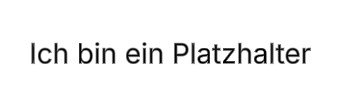
\includegraphics[width=0.3\linewidth]{inhalt/bilder/Platzhalter.jpg}
	\caption{Dargestelt ist der Schaltplan der Wortuhr mit allen angeschlossenen Komponenten und Pinbelegung des ESP32-C6.}
	\label{fig:Konzeptentwicklung}
\end{figure}

Zur Bestimmung der minimal nötigen Buchstabengröße wird ein empirischer Ansatz gewählt. 
Hierfür werden Testdrucke mit unterschiedlichen Schriftgrößen erstellt.
Das entscheidende Kriterium ist die gute Lesbarkeit aus einer Entfernung von etwa 5 m. 

Auf Basis der ermittelten Schriftgröße geht zum einen die Gesamtgröße der Wortuhr hervor.
Weiterhin kann damit der Abstand ermittelt und leicht angepasst werden, den die \gls{led}s voneinander haben müssen, damit eine \gls{led} je Buchstabe platziert wird.
Damit kann das passende \gls{led}-Band gewählt werden auf welchem die \gls{ws2812b}-\gls{led}s integriert sind.
So muss nicht jede \gls{led} einzeln verlötet werden.  
Zuletz bildet dies die Grundlage für die Aufteilung der Bauteile im Hinblick auf den Fertigungsprozess. 
Da das verfügbare Druckbett des verfügbaren \gls{3ddrucker} auf ein Volumen von 250 mm × 250 mm × 250 mm begrenzt ist, erfolgt eine entsprechende Segmentierung der Konstruktion und die Frontplattenbauteil können konstruiert werden.
    \section{Mechanische Konstruktion und Fertigung}
Die mechanische Basis des Systems bildet eine Multiplexplatte, die als tragende Struktur dient.  
Auf dieser Grundplatte werden die LED-Streifen montiert und die Frontabdeckung verschraubt.  
Der Mikrocontroller wird auf der Rückseite der Platte befestigt.  
Für die Darstellung der Wortmatrix werden Bauteile konstruiert und mittels \gls{3ddruck} aus schwarzem \gls{pla} hergestellt.
Ein Beispiel dafür ist in Abb.~\ref{fig:3DDruckbeispiel} dargestellt.
\begin{figure}[H]
	\centering
	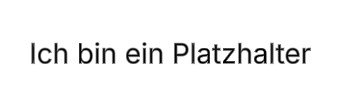
\includegraphics[width=0.3\linewidth]{inhalt/bilder/Platzhalter.jpg}
	\caption{Fertiggestellter Druck des Frontplattenbauteil Nr. 11 auf dem 3D-Drucker Kobra S1 der Marke Anycubic.}
	\label{fig:3DDruckbeispiel}
\end{figure}
Die gedruckten Bauteile bilden die Frontplatte sowie die Einhausung der LEDs.  
Die Konstruktion basiert auf einer modularen Struktur aus insgesamt 16 Einzelteilen (vgl. Abb.~\ref{fig:Frontplatte}), welche miteinander verschraubt werden.  
Dadurch entsteht eine zusammenhängende Frontabdeckung mit den Abmessungen H x B x T.    
\begin{figure}[H]
	\centering
	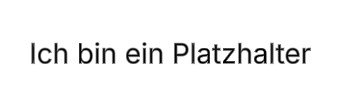
\includegraphics[width=0.3\linewidth]{inhalt/bilder/Platzhalter.jpg}
	\caption{}
	\label{fig:}
\end{figure}
Die Bauteile werden in drei Grundtypen unterteilt.  
Es existieren Mittelstücke, Eckstücke und Seitenstücke (vgl. Abb.~\ref{fig:Frontplatte}).  
Alle Bauteile folgen demselben konstruktiven Prinzip, unterscheiden sich jedoch in der jeweiligen Buchstabenbelegung oder Symbolik.  

Die Hauptanzeige, die aus 16 mal 16 Buchstaben besteht, dient der Darstellung der Uhrzeit, der Außentemperatur und des Wetters.  
Zusätzlich werden Symbole für die Zusatzfunktionen integriert, welche links, rechts, ober- und unterhalb der Buchstabenmatrix angeordnet sind (vgl. Abb.~\ref{fig:Frontplatte}).  
Diese umfassen die Anzeige von Raumfeuchtigkeit, Innenraumtemperatur, Mondphase und Tageszeit (vgl. Abb.~\ref{fig:ZusatzfunktionenaufderUhr}).  
\begin{figure}[H]
    \centering
    \begin{subfigure}[t]{0.48\textwidth}
        \centering
        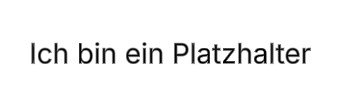
\includegraphics[width=\linewidth]{inhalt/bilder/Platzhalter.jpg}
        \caption{links oben}
        \label{fig:Raumfeuchtigkeit}
    \end{subfigure}
    \hfill
    \begin{subfigure}[t]{0.48\textwidth}
        \centering
        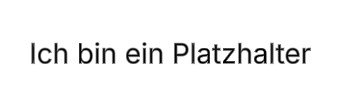
\includegraphics[width=\linewidth]{inhalt/bilder/Platzhalter.jpg}
        \caption{rechts oben}
        \label{fig:Innenraumtemperatur}
    \end{subfigure}
    \vspace{0.8em}
    \begin{subfigure}[t]{0.48\textwidth}
        \centering
        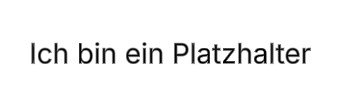
\includegraphics[width=\linewidth]{inhalt/bilder/Platzhalter.jpg}
        \caption{links unten}
        \label{fig:Mondphase}
    \end{subfigure}
    \hfill
    \begin{subfigure}[t]{0.48\textwidth}
        \centering
        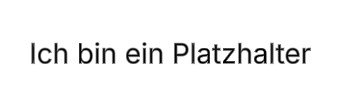
\includegraphics[width=\linewidth]{inhalt/bilder/Platzhalter.jpg}
        \caption{rechts unten}
        \label{fig:Tageszeit}
    \end{subfigure}
    \caption{Darstellung der vier Zusatzfunktionen die die Wortuhr neben der Uhrzeit, der Außentemperatur und dem Wetter anzeigen.}
    \label{fig:ZusatzfunktionenaufderUhr}
\end{figure}
Die Sekundenanzeig ist am Ausenrand der Frontplatte mit 60 Schlitzen realisiert (vgl. Abb.~\ref{fig:Frontplatte}).

Die Verbindung zur Grundplatte erfolgt über die Eckstücke.  
Hierzu werden Gewindeeinsätze, sogenannte Heatinsert, eingesetzt, welche in das 3D-gedruckte Material integriert werden (vgl. Abb.~\ref{fig:Heatinserts}).
Hierzu werden die Heatinserts z.B. mit einem Lötkolben mit geeigneter Spitze erhitzt und dann eingepresst.
\begin{figure}[H]
	\centering
	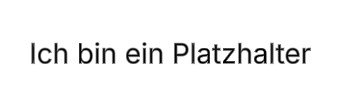
\includegraphics[width=0.3\linewidth]{inhalt/bilder/Platzhalter.jpg}
	\caption{}
	\label{fig:}
\end{figure}  
Die Befestigung erfolgt anschließend mit M4x20-Schrauben.  
Die Verbindung der einzelnen Frontbauteile untereinander erfolgt über Durchgangsbohrungen.  
Hierbei werden M3x12-Schrauben in Kombination mit Muttern und Unterlegscheiben verwendet.  

Zur Verbesserung der Lichtverteilung werden für jeden Buchstaben sowie jedes Symbol separate Diffusorplättchen eingesetzt.  
Diese werden ebenfalls im 3D-Druckverfahren aus weißem \gls{pla} hergestellt und dann eingeklebt.  
Die Plättchen besitzen eine Dicke von 0.4 mm, was einer Layerhöhe von 2 entspricht. 
Das bedeutet, der Drucker druckt nur 2 Schichten \gls{pla} übereinander.  
Die optimale Dicke wurde empirisch ermittelt, um eine gleichmäßige Lichtstreuung ohne signifikante Helligkeitsverluste zu erreichen.  
Zusätzlich wurden Bauteile als Abstandshalter zur Wand und gleichzeitig als Aufhängungspunkte konstruiert.   
Weiterhin wurde eine Montageplatte für den Mikrocontroller entwickelt, welche an der Rückseite der Multiplexplatte montiert ist.  
Dadurch bleibt die USB-C-Schnittstelle des Mikrocontroller auch im montierten Zustand erreichbar. 
\begin{figure}[H]
    \centering
    \begin{subfigure}[t]{0.32\textwidth}
        \centering
        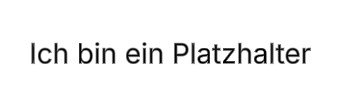
\includegraphics[width=\linewidth]{inhalt/bilder/Platzhalter.jpg}
        \caption{3D gedrucktes Diffusorplättchen mit einer dicke von 0,4 mm.}
        \label{fig:Diffusor}
    \end{subfigure}
    \hfill
    \begin{subfigure}[t]{0.32\textwidth}
        \centering
        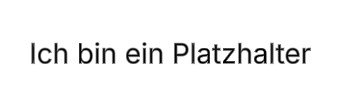
\includegraphics[width=\linewidth]{inhalt/bilder/Platzhalter.jpg}
        \caption{3D gedruckte Abstandshalter und Befestigungspunkte der Wortuhr.}
        \label{fig:Abstandshalter}
    \end{subfigure}
    \hfill
    \begin{subfigure}[t]{0.32\textwidth}
        \centering
        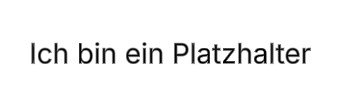
\includegraphics[width=\linewidth]{inhalt/bilder/Platzhalter.jpg}
        \caption{3D gedruckte Montageplatte für den ESP32-C6, welche an der Rückseite montiert wird.}
        \label{fig:MontageplatteESP}
    \end{subfigure}
\end{figure}
    \section{Installation der elektrischen Komponenten}
Die elektrische Installation basiert auf der Versorgungsspannung von 5 V.  
Alle LED-Streifen sowie der Mikrocontroller werden damit versorgt und haben einen gemeinsamen Ground.  

Es werden drei LED-Streifen eingesetzt. 
Der erste hat 256 \gls{ws2812b}-\gls{led}s und wird für die Anzeige von Stunden und Minuten, der Außentempreatur und dem Wetter verwendet.  
Der zweite hat 60 \gls{ws2812b}-\gls{led}s und wird für die Sekundenanzeige genutzt.
Der dritte hat 37 \gls{ws2812b}-\gls{led}s und wird für die Anzeige der Zusatzfunktionen genutzt.
Die Datenleitungen der LED-Streifen werden jeweils auf separate GPIO-Pins des Mikrocontrollers geführt.  

Die Dimensionierung des Netzteils erfolgt auf Basis der maximal möglichen Leistungsaufnahme.  
Die Gesamtleistung ergibt sich aus der maximalen Anzahl an LEDs die gleichzeitig aktiv sein können und deren spezifischer Leistungsaufnahme.  
Für die Berechnung kann folgende Beziehung verwendet werden:  
\[
P_{\text{gesamt}} = N_{\text{LED}} \cdot P_{\text{LED}}
\]

Die Leistungsaufnahme pro LED kann über die Streckenleistung bestimmt werden welche im Datenblatt der verwendeten \gls{led}-Streifen angegeben ist:  
\[
P_{\text{LED}} = \frac{P_{\text{pro Meter}}}{N_{\text{LED pro Meter}}}
\]

Für den verwendeten LED-Streifen ergeben sich laut Herstellerangaben eine Leistungsaufnahme von  
\[
P_{\text{pro Meter}} = 6\,\text{W/m}
\]
bei einer Bestückung von  
\[
N_{\text{LED pro Meter}} = 30\,\text{LED/m}
\]

Damit ergibt sich die Leistungsaufnahme einer einzelnen LED zu:  
\[
P_{\text{LED}} = \frac{6\,\text{W/m}}{30\,\text{LED/m}}
= 0{,}2\,\text{W}
\]

Im ungünstigsten Fall sind während des Boot-Modus kurzzeitig alle 256 LEDs des Hauptstreifens, bei voller Helligkeit, gleichzeitig aktiv. Daraus ergibt sich die maximale Gesamtleistung zu:  
\[
P_{\text{gesamt}} = 256 \cdot 0{,}2\,\text{W}
= 51{,}2\,\text{W}
\]

Die Stromaufnahme berechnet sich mit:  
\[
I_{\text{gesamt}} = \frac{P_{\text{gesamt}}}{U}
\]

Bei einer Versorgungsspannung von  
\[
U = 5\,\text{V}
\]
ergibt sich:  
\[
I_{\text{gesamt}} = \frac{51{,}2\,\text{W}}{5\,\text{V}}
= 10{,}24\,\text{A}
\]

Die mindestens erforderliche Netzteilleistung ergibt sich anschließend zu:  
\[
P_{\text{Netzteil}} = U \cdot I_{\text{gesamt}}
\]

Somit ergibt sich eine erforderliche Mindestleistung von:  
\[
P_{\text{Netzteil}} = 5\,\text{V} \cdot 10{,}24\,\text{A}
= 51{,}2\,\text{W}
\]

Obwohl im Boot-Modus kurzzeitig alle 256 LEDs des Hauptstreifens bei voller Helligkeit aktiviert werden, tritt dieser Zustand nur für etwa eine Sekunde auf. 
Für die thermische und dauerhafte Auslegung des Netzteils ist dieser kurzzeitige Spitzenwert nicht maßgebend.
Im normalen Betrieb sind deutlich weniger LEDs gleichzeitig aktiv. 
Der kurzzeitige Einschaltzustand während des Boot-Modus kann vom Netzteil als kurzzeitige Lastspitze bereitgestellt werden. 
Aus diesem Grund wird ein Netzteil mit einer Ausgangsstromstärke von \SI{10}{\ampere} bei \SI{5}{\volt} verwendet.
Mit diesem ist auch die Leistungsaufnahme des \gls{esp32c6} und des \gls{dht22} Sensors mit genügend Reserve abgedeckt.

In Abbildung~\ref{fig:Schaltplan} ist noch der Schaltplan der Wortuhr dargestellt.
\todo{Schaltplan}
\begin{figure}[H]
	\centering
	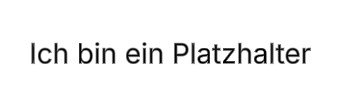
\includegraphics[width=0.3\linewidth]{inhalt/bilder/Platzhalter.jpg}
	\caption{Dargestelt ist der Schaltplan der Wortuhr mit allen angeschlossenen Komponenten und Pinbelegung des ESP32-C6.}
	\label{fig:Schaltplan}
\end{figure}
    \section{Aufbau der Wortuhr}
Nach der mechanischen und elektrischen Vorbereitung, der Konstruktion sowie dem \gls{3ddruck} der Bauteile, erfolgt die Montage des Gesamtsystems.  
Zunächst werden die LED-Streifen zugeschnitten und entsprechend der geplanten Anordnung auf die Grundplatte geklebt.
Hierzu wird das Layout auf die Grundplatte gezeichnet und die positionen der \gls{led}s mit dem zugehörigen Buchstaben bzw. Symbold und den Indizes der \gls{led} beschriftet.
Dadurch kann, ohne die aufgesetzte Frontplatte bei der Inbetriebnahme dauernd abzunehmen und wieder aufzusetzen überprüft werden, ob die korrekten Wörter angezeigt werden und die korrekte \gls{led} angsprochen wird.  
Anschließend werden die einzelnen Streifen durch Lötverbindungen verbunden (vgl. Abb~\ref{fig:VerlötetStreifen}).  
Die Anschluskabel werden auf die Rückseite geführt.  
\begin{figure}[H]
	\centering
	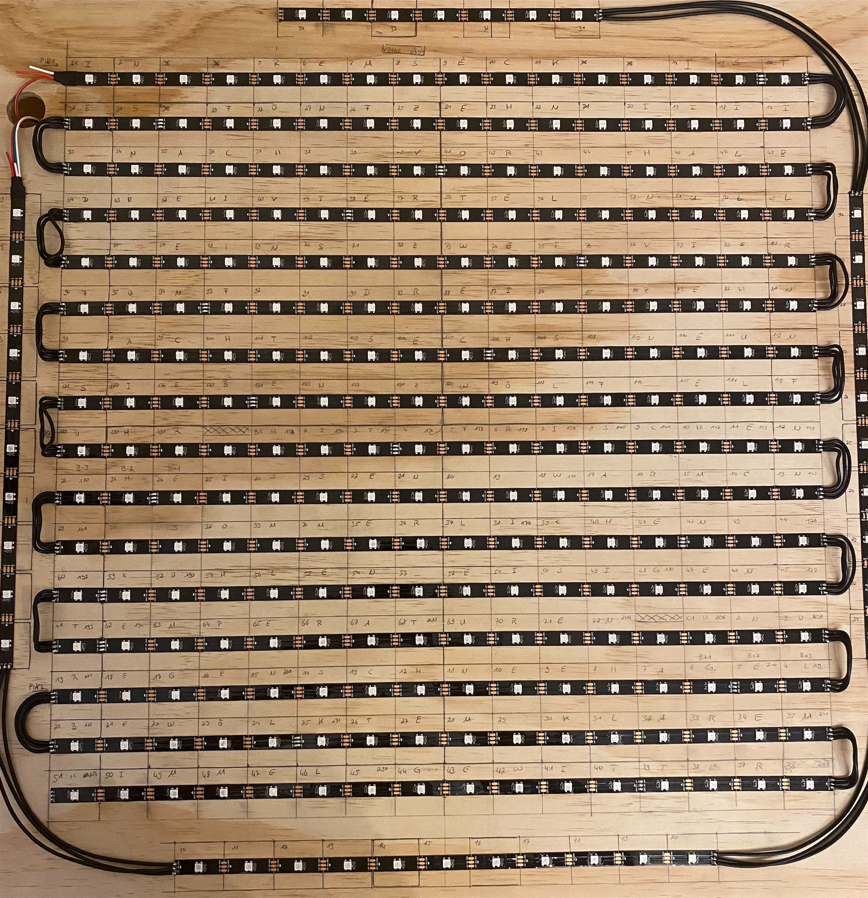
\includegraphics[width=0.7\linewidth]{inhalt/bilder/LEDsVerloetet.png}
	\caption{Alle LED-Streifen auf der Multiplexplatte aufgeklebt und verlötet.}
	\label{fig:VerlötetStreifen}
\end{figure}

Die Verbindung der Frontplatte zur Grundplatte erfolgt über die Eckstteile.  
Hierzu werden Gewindeeinsätze, sogenannte Heatinsert, eingesetzt, welche in das 3D-gedruckte Material integriert werden (vgl. Abb.~\ref{fig:Heatinserts}).
Hierzu werden die Heatinserts z.B. mit einem Lötkolben mit geeigneter Spitze erhitzt und dann eingepresst.
\begin{figure}[H]
	\centering
	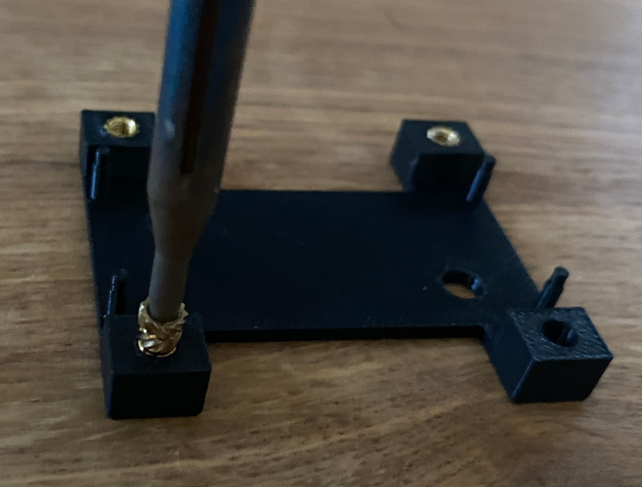
\includegraphics[width=0.7\linewidth]{inhalt/bilder/BeispielHeatinsertESPHalter.png}
	\caption{Einpressvorgang der der Heatinserts am Beispiel des ESP-Halters.}
	\label{fig:Heatinserts}
\end{figure}  
Die Befestigung erfolgt anschließend mit M4x20-Schrauben.  
Die Verbindung der einzelnen Frontplattenbauteile untereinander erfolgt über Durchgangsbohrungen.  
Hierbei werden M3x12-Schrauben in Kombination mit Muttern und Unterlegscheiben verwendet. 

Für die initiale Inbetriebnahme und implementierung der Software wird der Mikrocontroller provisorisch angeschlossen.  
Hierzu werden ein Steckbrett und Jumperkabel verwendet.  
Diese Vorgehensweise ermöglicht eine flexible Anpassung der Verdrahtung während der Testphase.
% Nach erfolgreicher Prüfung aller Funktionen erfolgt die finale Verdrahtung.  
% Die provisorischen Verbindungen werden durch dauerhafte Lötverbindungen ersetzt.
    \section{Implementierung der Software}
Die Softwareentwicklung erfolgt schrittweise und modular.  
Zunächst werden grundlegende Funktionen implementiert.  
Dazu zählen die Initialisierung der Hardware sowie die Ansteuerung der LED-Streifen.  
Die Ansteuerung der LEDs erfolgt über dedizierte Funktionen.  
Eine zentrale Funktion stellt die gezielte Aktivierung einzelner LEDs dar:  
\begin{verbatim}
void setLed(int ledNumber, uint8_t r, uint8_t g, uint8_t b)
<HIER KOMMT NOCH EIN CODEAUSSCHNITT HIN>
\end{verbatim}
Für die gleichzeitige Ansteuerung mehrerer LEDs werden Arrays verwendet.  
Diese enthalten die Indizes der LEDs, die ein bestimmtes Wort darstellen.  
Für Zeitanzeige, Temperaturinfos, Wetterinfis und Zusatzinformationen werden separate LED-Arrays definiert.  
Die Verarbeitung der Zeit erfolgt durch zyklisches Auslesen der Systemzeit.  
Die Anzeige wird in regelmäßigen Intervallen aktualisiert.  
Die Funktion zur Darstellung der Uhrzeit ist wie folgt aufgebaut:  
\begin{verbatim}
void showHourWord(int hour24)
<HIER KOMMT NOCH EIN CODEAUSSCHNITT HIN>
\end{verbatim}
Die Software wird iterativ aufgespielt und erweitert.  
Nach jeder Erweiterung erfolgt eine Funktionsprüfung.  
Dieses Vorgehen ermöglicht eine schrittweise Integration aller Systemfunktionen und verreinfacht die Fehlersuche bei Problemen.
    \section{Anbindung externer Datenquellen}
Zur Erweiterung der Funktionalität werden externe Datenquellen eingebunden.  
Die Kommunikation erfolgt über eine \gls{wlan}-Verbindung.  
Der Verbindungsaufbau wird durch eine eigene Funktion realisiert:  
\begin{verbatim}
void connectToWiFi()
<HIER KOMMT NOCH EIN CODEAUSSCHNITT HIN>
\end{verbatim}
Die Zeit wird über \gls{ntp} synchronisiert und die Wetterdaten von der Web-\gls{api} von Open-Meteo.
Die Synchronisation erfolgt initial beim Systemstart sowie zyklisch im Betrieb.   
Die Daten werden über \gls{https} abgerufen und im \gls{json}-Format verarbeitet.  
Die zentrale Funktion zur Aktualisierung der Wetterdaten lautet:  
\begin{verbatim}
bool updateWeatherFromServer()
<HIER KOMMT NOCH EIN CODEAUSSCHNITT HIN>
\end{verbatim}
Die empfangenen Daten werden anschließend klassifiziert.  
Hierzu werden die Temperaturwerte über eine Case-Anweisung ausgewählt und der Wettercode in eine definierte Wettergruppe überführt.
Mit dieser wird dann ebenfalls über eine Case-Anweisung die aktuelle Wetteranzeige ausgewählt.
Die Anzeige erfolgt dann durch Zuordnung zu entsprechenden Wörtern welche als Globale Variablen deklariert sind.
    \section{Integration der mobile Steuerung}
% Zur Steuerung des Systems wird ein integrierter Webserver implementiert, welcher direkt auf dem Mikrocontroller läuft.  
% Die Kommunikation erfolgt über HTTP und der Zugriff ist über einen Webbrowser möglich.  

% Dabei übernimmt eine zentrale Funktion die Generierung der HTML-Benutzeroberfläche:

% \begin{lstlisting}[style=arduino, caption={Generierung der HTML-Benutzeroberflaeche}]
% String buildHtmlPage() {
%   String colorHex = rgbToHex(ledR, ledG, ledB);

%   String html = "";
%   html += "<!DOCTYPE html><html><head><meta charset='utf-8'>";
%   html += "<meta name='viewport' content='width=device-width, initial-scale=1'>";
%   html += "<title>WordClock</title>";

%   html += "<style>";
%   html += "body{font-family:Arial,sans-serif;background:#111;color:#eee;margin:20px;}";
%   html += "h1{color:#fff;}";
%   html += ".card{background:#1e1e1e;padding:16px;border-radius:12px;margin-bottom:16px;}";
%   html += "</style>";

%   html += "</head><body>";
%   html += "<h1>WordClock</h1>";

%   html += "<div class='card'>";
%   html += "<h2>Steuerung</h2>";
%   html += "<a href='/set?power=1'>EIN</a>";
%   html += "<a href='/set?power=0'>AUS</a>";
%   html += "</div>";

%   html += "</body></html>";

%   return html;
% }
% \end{lstlisting}

% Die Benutzeroberfläche ermöglicht die Steuerung zentraler Parameter.  
% Dazu zählen Ein- und Ausschalten, Helligkeit sowie Farbwerte.  

% Die Verarbeitung der Nutzereingaben erfolgt über URL-Parameter.  
% Diese werden durch eine entsprechende Handler-Funktion ausgewertet.  
% Zusätzlich wird eine JSON-Schnittstelle bereitgestellt.  
% Diese erlaubt den Zugriff auf Statusinformationen für externe Anwendungen.

% Die Benutzeroberfläche ist in Abbildung~\ref{fig:Benutzeroberflaeche} dargestellt.

% \begin{figure}[H]
%     \centering
%     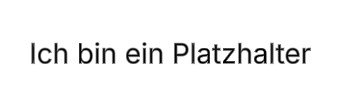
\includegraphics[width=0.3\linewidth]{inhalt/bilder/Platzhalter.jpg}
%     \caption{HTML-Benutzeroberfläche der Wortuhr. Über diese können die Wortuhr ein- und ausgeschaltet, die Helligkeit angepasst und die Farbe der LEDs verändert werden. Weiterhin können aktuelle Statusinformationen der Wortuhr überwacht werden.}
%     \label{fig:Benutzeroberflaeche}
% \end{figure}

Zur Steuerung des Systems wird ein integrierter Webserver implementiert, welcher direkt auf dem Mikrocontroller ausgeführt wird.  
Die Kommunikation erfolgt über HTTP und der Zugriff ist über einen Webbrowser möglich.
Die Benutzeroberfläche ermöglicht das Ein- und Ausschalten der Wortuhr sowie die Anpassung von Helligkeit und Farbwerten.  
Die Verarbeitung der Nutzereingaben erfolgt über URL-Parameter.

\begin{lstlisting}[style=arduino,caption={Verarbeitung der Nutzereingaben ueber URL-Parameter}]
void handleSet() {
  bool changed = false;

  if (server.hasArg("power")) {
    int p = server.arg("power").toInt();
    lampPower = (p != 0);
    changed = true;
  }

  if (server.hasArg("brightness")) {
    int b = server.arg("brightness").toInt();

    if (b < 0) b = 0;
    if (b > 100) b = 100;

    webBrightness = b;
    changed = true;
  }

  if (changed) {
    showHourWord(currentHour);
  }

  server.sendHeader("Location", "/", true);
  server.send(302, "text/plain", "OK");
}
\end{lstlisting}

Zusätzlich wird eine JSON-Schnittstelle bereitgestellt, über welche Statusinformationen für externe Anwendungen ausgelesen werden können.  
Die HTML-Benutzeroberfläche wird dynamisch auf dem ESP32 erzeugt und über den integrierten HTTP-Server bereitgestellt.  
Weitere Funktionen zur Generierung der HTML-Seite, API-Ausgabe und Verarbeitung von Browseranfragen befinden sich im vollständigen Programmcode in Anhang~\ref{apx:1}.  

Die Benutzeroberfläche kann als Web-App direkt zum Homebildschirm eines mobilen Endgeräts hinzugefügt werden.  
Dadurch lässt sich die Steuerung der Wortuhr ähnlich wie eine native Smartphone-Anwendung bedienen (vgl. Abbildung~\ref{fig:APIHomebildschirm}).

\begin{figure}[H]
    \centering
    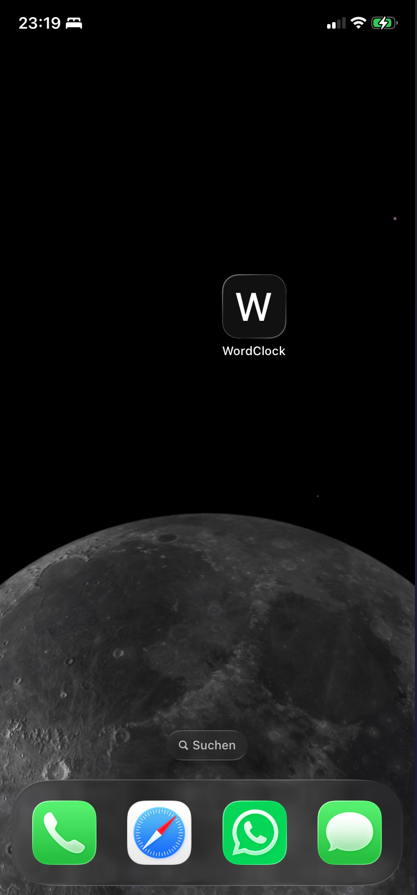
\includegraphics[width=0.4\linewidth]{inhalt/bilder/APIHomebildschirm.png}
    \caption{Die HTML-Benutzeroberfläche kann als Web-App zum Homebildschirm hinzugefügt werden und ermöglicht dadurch einen schnellen Zugriff auf die Steuerung der Wortuhr.}
    \label{fig:APIHomebildschirm}
\end{figure}

Nach dem Öffnen der Benutzeroberfläche werden zunächst die aktuellen Statusinformationen der Wortuhr angezeigt.  
Hierzu zählen unter anderem Uhrzeit, Wetterdaten, Helligkeit, Farbwerte sowie Sensorinformationen (vgl. Abbildung~\ref{fig:APIParameteruebersicht}).

\begin{figure}[H]
    \centering
    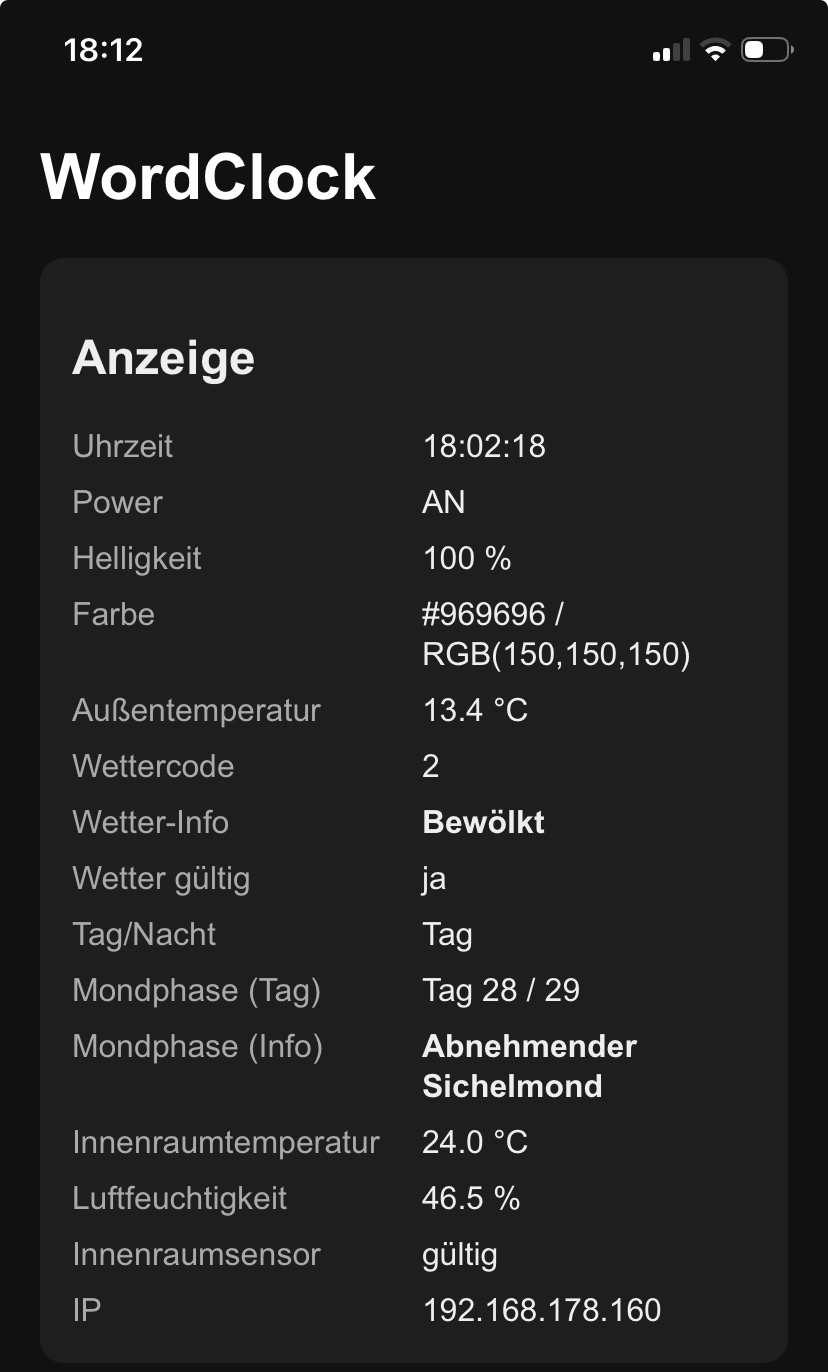
\includegraphics[width=0.4\linewidth]{inhalt/bilder/APIParameterübersicht.png}
    \caption{Übersicht der aktuellen Systemparameter und Statusinformationen innerhalb der HTML-Benutzeroberfläche.}
    \label{fig:APIParameteruebersicht}
\end{figure}

Im unteren Bereich der Benutzeroberfläche befinden sich die Bedienelemente.  
Über diese kann die Wortuhr ein- und ausgeschaltet sowie eine manuelle Aktualisierung der Wetterdaten ausgelöst werden (vgl. Abbildung~\ref{fig:APIEinAus}).

\begin{figure}[H]
    \centering
    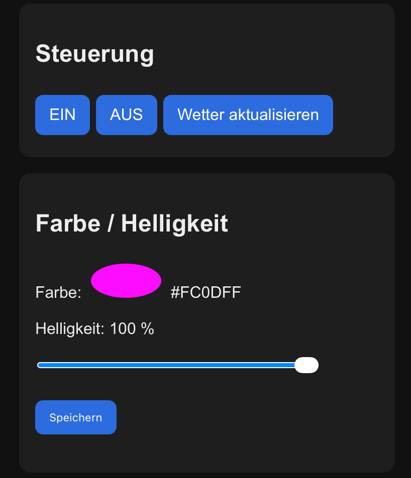
\includegraphics[width=0.4\linewidth]{inhalt/bilder/APIEINAUSFARBE.png}
    \caption{Bedienelemente der HTML-Benutzeroberfläche zur Steuerung der Wortuhr und zur Aktualisierung der Wetterinformationen.}
    \label{fig:APIEinAus}
\end{figure}

Zusätzlich können Helligkeit und Farbe der LED-Beleuchtung angepasst werden.  
Die Helligkeit wird über einen Slider eingestellt, während die Farbe über einen integrierten Farbwähler ausgewählt werden kann (vgl. Abbildung~\ref{fig:APIFarbe}).

\begin{figure}[H]
    \centering
    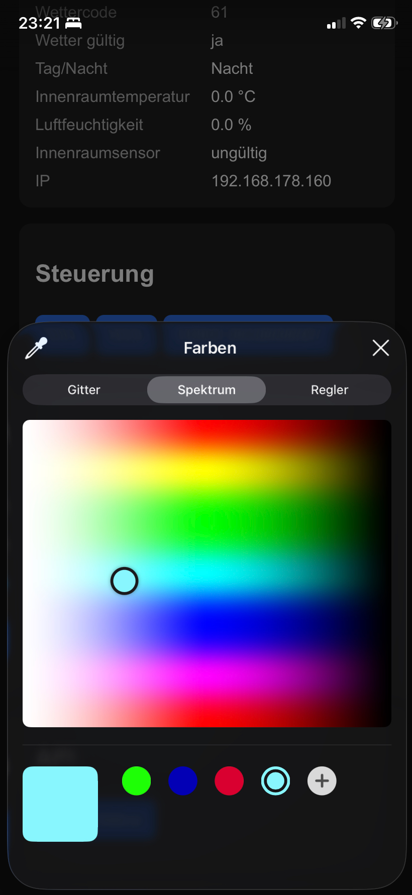
\includegraphics[width=0.4\linewidth]{inhalt/bilder/APIFarbe.png}
    \caption{Einstellmöglichkeiten für Helligkeit und Farbe der LED-Beleuchtung innerhalb der mobilen Benutzeroberfläche.}
    \label{fig:APIFarbe}
\end{figure}

% Zusätzlich wird eine JSON-Schnittstelle bereitgestellt, über welche Statusinformationen für externe Anwendungen ausgelesen werden können.  
% Die HTML-Benutzeroberfläche wird dynamisch auf dem ESP32 erzeugt und über den integrierten HTTP-Server bereitgestellt.
% Weitere Funktionen zur Generierung der HTML-Seite, API-Ausgabe und Verarbeitung von Browseranfragen befinden sich im vollständigen Programmcode in Anhang~\ref{apx:1}.
% Die Benutzeroberfläche und verwendung dieser ist in Abbildung~\ref{fig:Benutzeroberflaeche} dargestellt.

% \begin{figure}[H]
%     \centering
%     \begin{subfigure}[t]{0.3\textwidth}
%         \centering
%         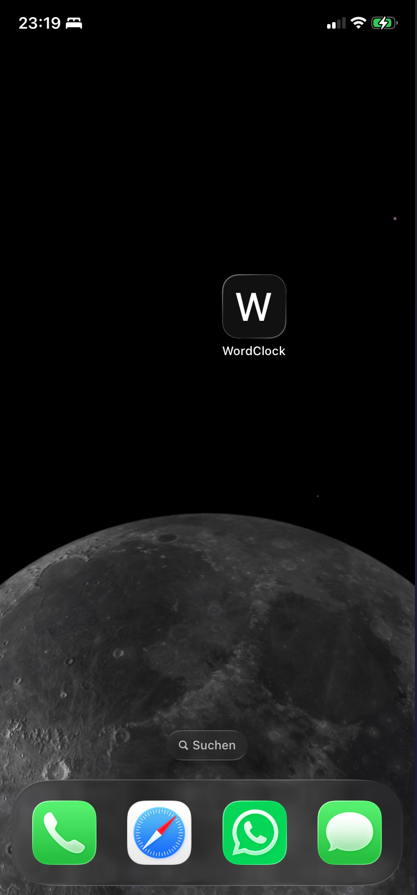
\includegraphics[width=\linewidth]{inhalt/bilder/APIHomebildschirm.png}
%         \caption{Die HTML-Benutzeroberfläche kann als Web App zum Homebildschirm hinzugefügt werden wodurch sich die API wie eine App öffnen und bedienen lässt.}
%         \label{fig:sub_a}
%     \end{subfigure}
%     \hfill
%     \begin{subfigure}[t]{0.4\textwidth}
%         \centering
%         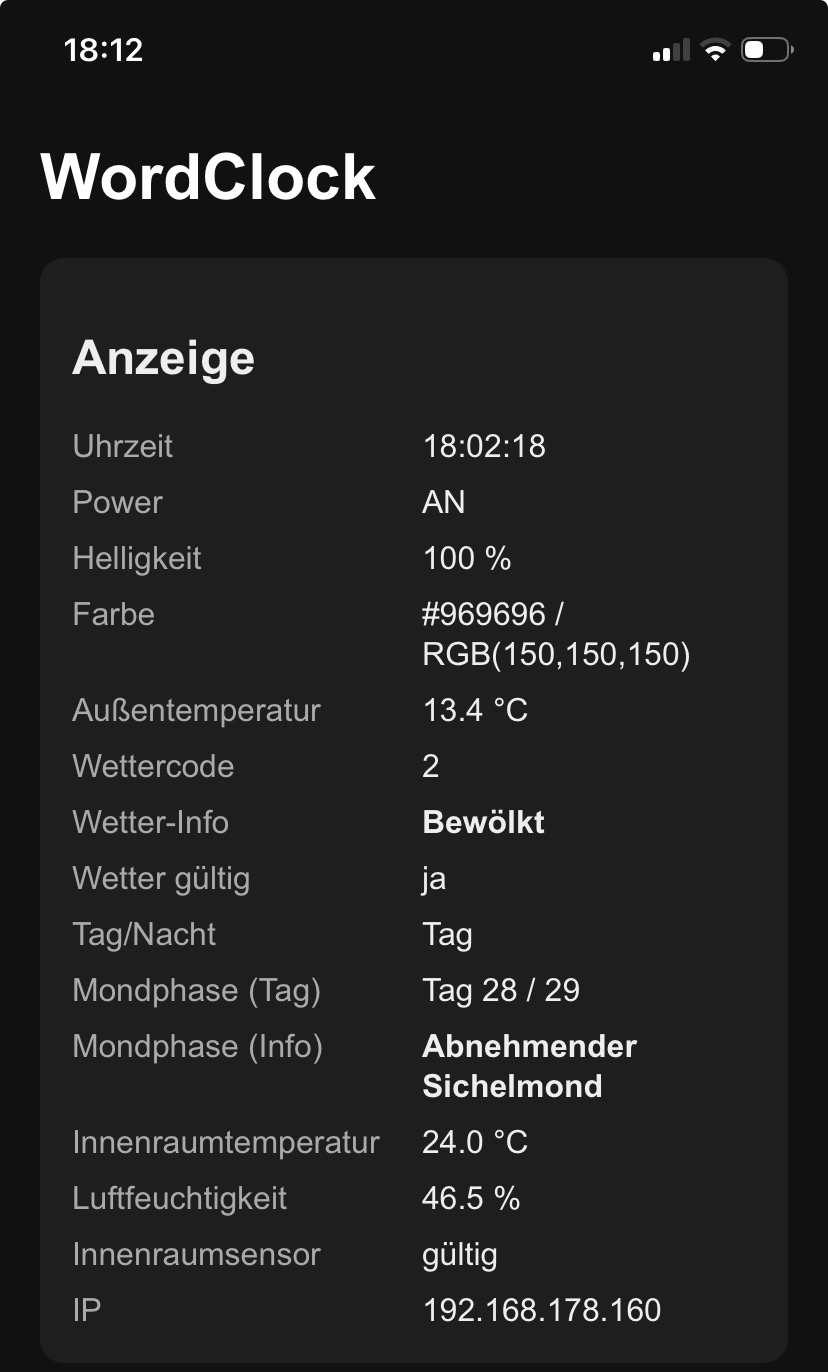
\includegraphics[width=\linewidth]{inhalt/bilder/APIParameterübersicht.png}
%         \caption{Beim öffnen der API sieht man im oberen Teil zunächst eine Übersicht aller Variablen und deren aktuelle Werte.}
%         \label{fig:sub_b}
%     \end{subfigure}
%     \vspace{0.8em}
%     \begin{subfigure}[t]{0.4\textwidth}
%         \centering
%         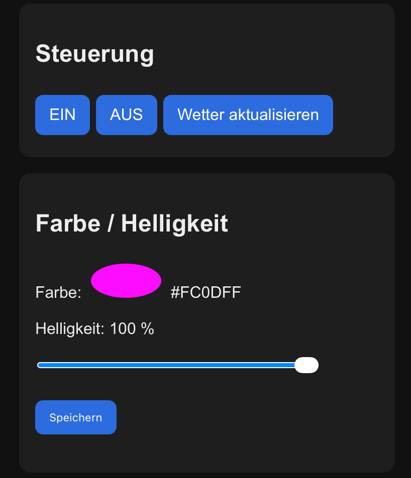
\includegraphics[width=\linewidth]{inhalt/bilder/APIEINAUSFARBE.png}
%         \caption{Im unteren Teil sieht man die Bedienflächen um die Wortuhr ein- und auszuschalten, sowie eine aktualisierung der Wetterinformationen zu initialisieren. Darunter befindet sich die Schaltfläche für die Farb- und Helligkeitssteuerung.}
%         \label{fig:sub_c}
%     \end{subfigure}
%     \hfill
%     \begin{subfigure}[t]{0.4\textwidth}
%         \centering
%         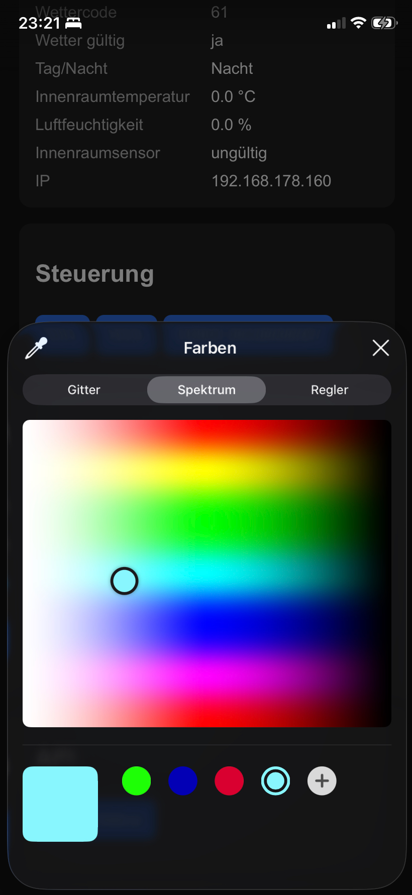
\includegraphics[width=\linewidth]{inhalt/bilder/APIFarbe.png}
%         \caption{Die Helligkeit lässt sich über den Slider regeln. Für die Farbeinstellung kommt man in dieses Fenster und kann die gewünschte Farbe auswählen. Zusätzlich kann man sich im unteren Teil Favoriten abspeichern.}
%         \label{fig:sub_d}
%     \end{subfigure}
%     \caption{HTML-Benutzeroberfläche der Wortuhr. Über diese können die Wortuhr ein- und ausgeschaltet, die Helligkeit angepasst und die Farbe der LEDs verändert werden. Zusätzlich lassen sich aktuelle Statusinformationen überwachen.}
%     \label{fig:Benutzeroberflaeche}
% \end{figure}


%   _________Kapitel 6_________
\input{inhalt/textkapitel/Kapitel 6/600_Test und Evaluation.tex}
    \section{Testkonzept und Vorgehensweise} \todo{7.1 + Abkürzungscheck}
Wie getestet wurde
Warum diese Tests gewählt wurden
    \section{Modultests} \todo{7.2 + Abkürzungscheck}
Einzelne Funktionen/Module werden getestet
Soll-/Ist-Vergleich
    \section{Integrationstests} \todo{7.3 + Abkürzungscheck}
Zusammenspiel der Komponenten prüfen
    \section{Systemtests und Dauerbetrieb} \todo{7.4 + Abkürzungscheck}
Nach erfolgreicher Integration aller Komponenten erfolgt die Prüfung des Gesamtsystems im Dauerbetrieb.  
Dabei werden Stabilität, Temperaturverhalten und Zuverlässigkeit untersucht.  

Das System wird zunächst über einen Zeitraum von mehreren Stunden betrieben.  
Währenddessen erfolgt wiederholt die Kontrolle der Zeit-, Wetter- und Temperaturanzeigen.  
Die angezeigte Uhrzeit wird regelmäßig mit einer externen Referenz verglichen.  
Dabei kann keine sichtbare zeitliche Abweichung festgestellt werden.  
Zusätzlich wird überprüft, ob sich elektronische Komponenten oder Leitungen unzulässig erwärmen.  
Während des Betriebs treten keine kritischen Temperaturentwicklungen auf.  

Anschließend erfolgt ein Dauerbetrieb über drei Tage.  
Dabei wird die Funktion der Wortuhr in regelmäßigen Abständen kontrolliert.  
Alle Anzeigen arbeiten während dieses Zeitraums stabil und fehlerfrei.  
Nach erfolgreichem Abschluss der Dauerlauftests erfolgt der Aufbau der finalen Hardwareversion.  
Die zuvor verwendeten Breadboard- und Jumperleitungen werden durch fest verlötete Leitungen ersetzt.  
Zusätzlich werden die entwickelten und gedruckten Halterungen und Befestigungselemente montiert.  

Nach der Endmontage erfolgt eine erneute Überprüfung aller Funktionen und elektrischen Verbindungen.  
Dabei wird kontrolliert, ob alle Anzeigen korrekt arbeiten und sämtliche Leitungen ordnungsgemäß verbunden sind.  
Nach erfolgreichem Abschluss der Systemtests wird die Wortuhr an ihrem vorgesehenen Einsatzort montiert und in Betrieb genommen.
    \section{Abnahme} \todo{7.5 + Abkürzungscheck}
Die Abnahme erfolgt durch einen abschließenden Vergleich der umgesetzten Funktionen mit den zuvor definierten Anforderungen.  

Die Wortuhr erfüllt die grundlegenden Anforderungen an die Anzeige der Uhrzeit in Wortform.  
Zusätzlich werden Wetterinformationen, Außentemperatur, Innenraumtemperatur, Luftfeuchtigkeit, Mondphase und Tageszeit dargestellt.  
Die WLAN-Anbindung sowie die Synchronisation über NTP arbeiten zuverlässig.  
Auch die mobile Steuerung über die HTML-Benutzeroberfläche funktioniert stabil.  
Die LED-Anzeigen besitzen eine gleichmäßige Helligkeit und eine stabile Farbdarstellung.  
Die Reaktionszeiten der Benutzeroberfläche sind kurz und ermöglichen eine komfortable Bedienung.    

Schwerwiegende Einschränkungen im Betrieb können bislang nicht festgestellt werden. 
Lediglich die Mondphasenberechnung und die Darstellung mit nur sechs Zuständen, kann geringfügige Abweichungen zur tatsächlichen Mondphase aufweisen.  
Insgesamt zeigt die Evaluation, dass die entwickelte Wortuhr die definierten Anforderungen erfüllt und im praktischen Betrieb zuverlässig arbeitet.


%   _________Kapitel 7_________
\input{inhalt/textkapitel/Kapitel 7/700_Diskussion der Ergebnisse.tex}
    \section{Erfüllung der Zielsetzung} \todo{8.1 + Abkürzungscheck}
Abgleich:
Ziele aus Kap. 1.2
Ergebnisse aus Kap. 6
    \section{Technische und gestalterische Bewertung} \todo{8.2 + Abkürzungscheck}
Kritische Reflexion:
Was ist gelungen?
Wo gab es Kompromisse?
    \section{Grenzen der Umsetzung} \todo{8.3 + Abkürzungscheck}
Technische Grenzen
Zeitliche Grenzen
Methodische Grenzen


%   _________Kapitel 8_________
\input{inhalt/textkapitel/Kapitel 8/800_Fazit und Ausblick.tex}
    \section{Zusammenfassung der Arbeit} \todo{9.1 + Abkürzungscheck}
Im Rahmen dieser Arbeit wurde eine Wortuhr mit erweiterten Zusatz- und Informationsfunktionen konzipiert, entwickelt und aufgebaut. 
Ziel war die Kombination der klassischen sprachbasierten Zeitdarstellung mit zusätzlichen technischen Funktionen innerhalb eines einheitlichen Gesamtsystems.

Zu Beginn der Arbeit wurden bestehende Konzepte analysiert und die funktionalen sowie technischen Anforderungen definiert. 
Darauf aufbauend erfolgte die Entwicklung der Hardwarearchitektur, der Softwarestruktur sowie der mechanischen Konstruktion. 
Die einzelnen Komponenten wurden anschließend zu einem funktionsfähigen Prototyp integriert.

Die entwickelte Wortuhr ermöglicht neben der sprachlichen Zeitdarstellung die Anzeige weiterer Informationen. 
Hierzu zählen Wetterdaten, Temperaturwerte, Luftfeuchtigkeit, Mondphasen sowie sekundengenaue Anzeigeelemente. 
Zusätzlich wurde eine netzwerkbasierte Kommunikation umgesetzt. 
Dadurch ist eine Steuerung über mobile Endgeräte möglich.

Die Arbeit zeigt, dass die Integration zusätzlicher Funktionen in eine Wortuhr technisch realisierbar ist. 
Gleichzeitig konnte eine Kombination aus funktionaler Informationsdarstellung und gestalterischer Ausführung erreicht werden.
    \section{Kritische Reflexion des Projekts} \todo{9.2 + Abkürzungscheck}
Lessons learned
    \section{Erweiterungs- und Verbesserungspotenziale} \todo{9.3 + Abkürzungscheck}
technische Verbesserungen
Zukunftsperspektiven nennen
weitere mögliche Funktionen

    
%   _________Kapitel Beispiel_________
%% !TeX root = ../main.tex
% Zeile 1 legt fest das immer die main.tex kompiliert wird

%% Beispiele, können problemlos entfernt werden!
\chapter{Beispiele und HowTo}
\todo{Kapitel auskommentieren vor Abgabe}

% ==========================================================================================================
\section{Verlinkung}
Strg+linke Maustaste an dieser Stelle im PDF um an die Stelle in tex zu springen.

% ==========================================================================================================
\section{Literatur}
Beispiel Text \cite[S. 10]{testBuch}
Beispiel Homepage \cite{testWebsite}

% ==========================================================================================================
\section{Bilder}
% ======================
\subsection{Einfaches Bild}
\begin{figure}[H]
	\centering
	
\includegraphics[width=0.3\linewidth]{inhalt/bilder/logo-dhbw.png}
	\caption{DHBW Logo}
	\label{fig:logo-dhbw}
\end{figure}

% ======================
\subsection{Doppelbild}
\begin{figure}[H]%\centering
	\begin{subfigure}{0.5\textwidth}
		\centering
		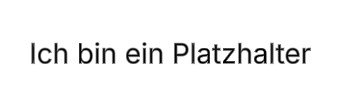
\includegraphics[width=\textwidth]{inhalt/bilder/Platzhalter.jpg}
		\caption{}\label{fig:Inv_Modul1}
	\end{subfigure}
	\hfill
	%\vspace{1em} % Abstand zwischen den Subfigures
	\begin{subfigure}{0.5\textwidth}
		\centering
		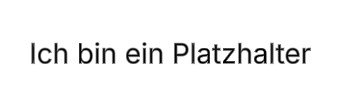
\includegraphics[width=\textwidth]{inhalt/bilder/Platzhalter.jpg}
		\caption{}\label{fig:Inv_Modul2}
	\end{subfigure}
	\caption{Caption, wenn untercaptions leer, automatisch durchnummeriert mit a und b}\label{fig:InverterModule}
\end{figure}

% ======================
\subsection{Multibild}
\begin{figure}[H]
    \centering
    \begin{subfigure}[t]{0.48\textwidth}
        \centering
        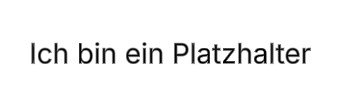
\includegraphics[width=\linewidth]{inhalt/bilder/Platzhalter.jpg}
        \caption{links oben}
        \label{fig:sub_a}
    \end{subfigure}
    \hfill
    \begin{subfigure}[t]{0.48\textwidth}
        \centering
        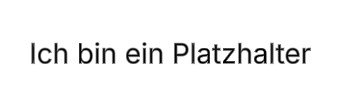
\includegraphics[width=\linewidth]{inhalt/bilder/Platzhalter.jpg}
        \caption{rechts oben}
        \label{fig:sub_b}
    \end{subfigure}
    \vspace{0.8em}
    \begin{subfigure}[t]{0.48\textwidth}
        \centering
        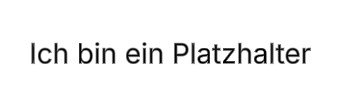
\includegraphics[width=\linewidth]{inhalt/bilder/Platzhalter.jpg}
        \caption{links unten}
        \label{fig:sub_c}
    \end{subfigure}
    \hfill
    \begin{subfigure}[t]{0.48\textwidth}
        \centering
        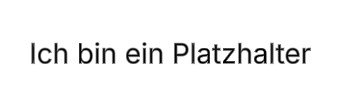
\includegraphics[width=\linewidth]{inhalt/bilder/Platzhalter.jpg}
        \caption{rechts unten}
        \label{fig:sub_d}
    \end{subfigure}
    \caption{Gesamte Bild Caption}
    \label{fig:GesBildCaption}
\end{figure}

% ======================
\subsection{Bildverweis}
Das Logo der DHBW (vgl. Abb.~\ref{fig:logo-dhbw})

% ==========================================================================================================
\section{Fußnote und Abkürzungen}
Fußnote\footnote{Fußnotenbeispiel}\\ Ersters mal \gls{DHBW} und zweites mal \gls{DHBW}

% ==========================================================================================================
\section{Tabellen}

% ======================
\subsection{einzeltabelle}
\begin{table}[H]
	\centering
	\caption{Tabellenbeispiel}
	\label{tab:example}
	\begin{tabular}{|l|c|r|}
		\hline
		Spalte 1 & Spalte 2 & Spalte 3 \\
		\hline
		Zeile  &  &  \\
		\hline
		& Zeile &  \\
		\hline
		&  & Zeile \\
		\hline
		\multicolumn{2}{|r|}{Verbunden}	& nicht Verbunden \\
		\hline
	\end{tabular}
\end{table}

% ======================
\subsection{doppeltabelle}
\begin{table}[H]
\centering
\begin{minipage}[t]{0.48\textwidth}
\centering
\caption{Vergleich der Kamerapositionen}
\label{tab:compare_per_camera}
\begin{tabular}{|l|c|c|c|c|}
\hline
Pos. & Test 1 & Test 2 & Test 3 & Test 4 \\
\hline
A & 100.00 & 81.48 & 100.00 & 100.00 \\
B & 55.56 & 59.26 & 100.00 & 100.00 \\
C & 100.00 & 87.04 & 100.00 & 96.30 \\
D & 100.00 & 100.00 & 100.00 & 100.00 \\
\hline
\end{tabular}
\end{minipage}\hspace{1em}
\begin{minipage}[t]{0.48\textwidth}
\centering
\caption{Vergleich der Klassen}
\label{tab:compare_per_class}
\begin{tabular}{|l|c|c|c|c|}
\hline
Klasse & Test 1 & Test 2 & Test 3 & Test 4 \\
\hline
gut & 25.00 & 25.00 & 41.67 & 25.00 \\
def. & 75.00 & 75.00 & 45.83 & 25.00 \\
falsch & 55.00 & 57.50 & 100.00 & 94.17 \\
offen & 70.83 & 50.00 & 87.50 & 87.50 \\
besch. & 0.00 & 20.83 & 75.00 & 95.83 \\
\hline
\end{tabular}
\end{minipage}
\end{table}

% ======================
\subsection{Quertabelle}
\begin{landscape}
    Text über Tabelle \ref{tab:breitetabelle}.
	\begin{table}[H]
		\caption{Breites Tabellenbeispiel}
		\label{tab:breitetabelle}
		\centering
		\resizebox{\columnwidth}{!}{%
			\begin{tabular}{|p{10cm}|p{10cm}|p{10cm}|}
				\hline
				Sehr & breite & Tabelle \\
				\hline
				\multicolumn{3}{|c|}{Tabelle wurde in der Größe verkleinert} \\
				\hline
			\end{tabular}
		}
	\end{table}
	Text unter Tabelle \ref{tab:breitetabelle}.
\end{landscape}

% ==========================================================================================================
\section{Skript}

% ======================
\lstinline[language=c]|printf("Inline Code");|

% ======================
\lstinputlisting[language=python,caption={Beispiel python Skript},captionpos=t,label=scr:example]{beispiele und befehle/example-script.py}

% ======================
\lstinputlisting[
	language=python,
	caption={Beispiel python Skript teilweise},
	captionpos=t,
	label=scr:example2,
	firstline=2,
	lastline=3
]{beispiele und befehle/example-script.py}

% ==========================================================================================================
\section{Skriptverweis}
Das Hallo Welt Skript (vgl. Skript~\ref{scr:example})

% ==========================================================================================================
\section{TODOs}
Text \todo{Dieser Text ist Randnotiz}

% ==========================================================================================================
\section{Auflistungen}
\begin{enumerate}
	\item Aufzählung nummeriert
\end{enumerate}

\begin{itemize}
	\item Aufzählung Stichpunkte
\end{itemize}

\begin{description}[style=nextline]
	\item[Label] Aufzählung als Beschreibung
\end{description}

Vorteile sind:
\begin{itemize}[noitemsep, topsep=0pt, partopsep=0pt, parsep=0pt]
  \item Anders
\end{itemize}

Nachteile sind:
\begin{itemize}[noitemsep, topsep=0pt, partopsep=0pt, parsep=0pt]
  \item Anders
\end{itemize}

\noindent
\begin{minipage}[t]{0.48\textwidth}
  \textbf{Vorteile}
  \begin{itemize}[nosep]
    \item Anders
  \end{itemize}
\end{minipage}\hfill
\begin{minipage}[t]{0.48\textwidth}
  \textbf{Nachteile}
  \begin{itemize}[nosep]
    \item Anders
  \end{itemize}
\end{minipage}